\documentclass[a4paper,landscape,pdftex]{article}

\usepackage[boldmath,widetext]{nvefoil}

\Trtitle{Wetenschapsweek}
\author{Nick van Eijndhoven}
\date{Vrije Universiteit Brussel (VUB)}

\lhead{\includegraphics[keepaspectratio,height=1.7cm]{vublogo-hor}}
\rhead{\includegraphics[keepaspectratio,height=2.3cm]{icecubelogo}}

\begin{document}

\begin{titlepage}
\begin{center}
\vspace*{-4cm}
\Title[20cm]{yellow}{blue}{IceCube : Neutrino's vangen op Antarctica}
{\LARGE \bf
 Nick van Eijndhoven\\[1mm]
 nick@icecube.wisc.edu $\quad$ http://www.iihe.ac.be\\[1cm]
 \includegraphics[keepaspectratio,height=2cm]{vublogo-hor} $\qquad$
 \includegraphics[keepaspectratio,height=2cm]{iihelogo}\\[3mm]
 Vrije Universiteit Brussel - IIHE(ULB-VUB)\\[1mm]
 Pleinlaan 2, B-1050 Brussel, Belgium
}
\end{center}
\Contscb{yellow}{blue}{Overzicht}{blue}
\end{titlepage}

\twocolumn

\Transcb{yellow}{blue}{Het zichtbare heelal}
\twocolumn
\begin{center}
{\blue Electromagnetische straling}\\[5mm]
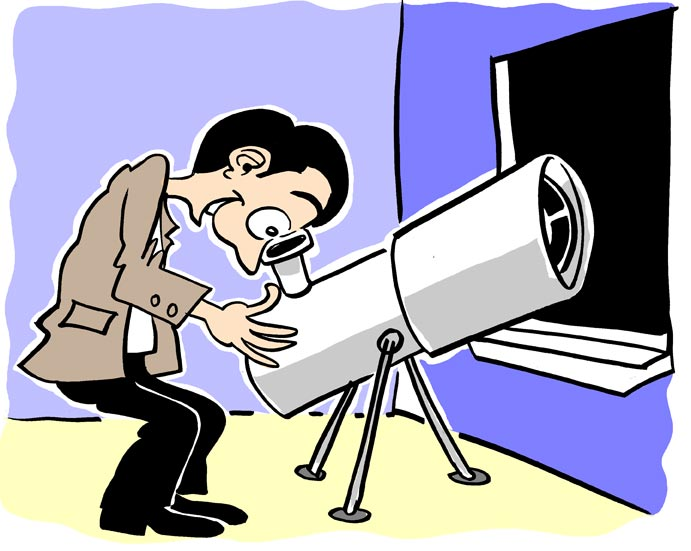
\includegraphics[keepaspectratio,width=5cm]{optical2}
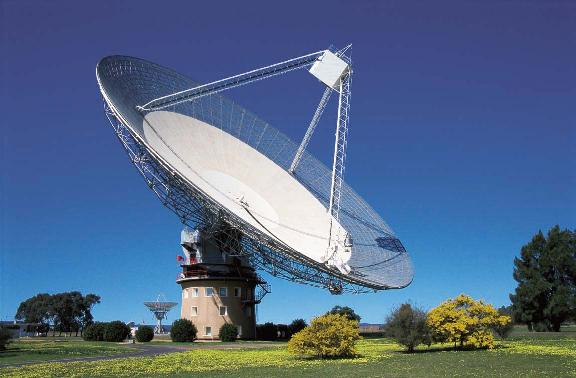
\includegraphics[keepaspectratio,width=7cm]{radio2}\\[1.5cm]
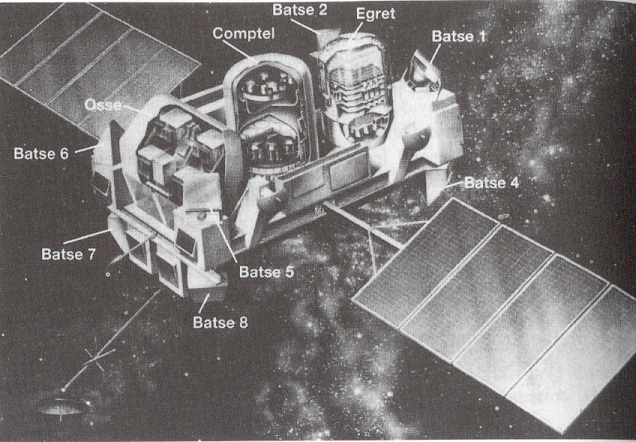
\includegraphics[keepaspectratio,width=12cm]{cgro}
\end{center}

\newpage

\begin{center}
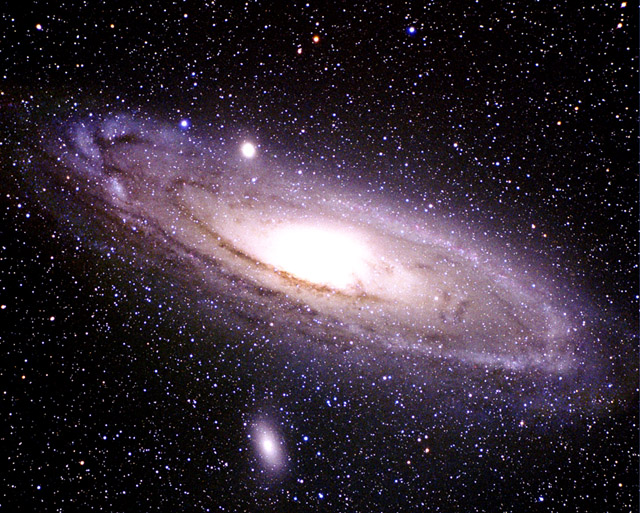
\includegraphics[keepaspectratio,height=7cm]{m31}\\[3mm]
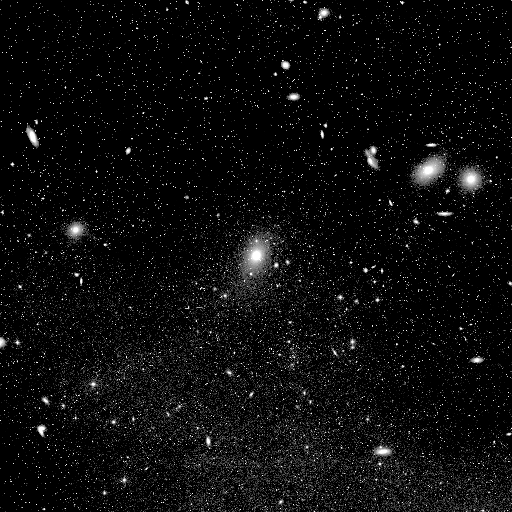
\includegraphics[keepaspectratio,height=8cm]{virgo}
\end{center}

\Tr
\vspace*{1mm}
\begin{itemize}
\item \colorbox{yellow}{Waar komt deze materie vandaan ?}
\end{itemize}
%
\vspace*{1cm}
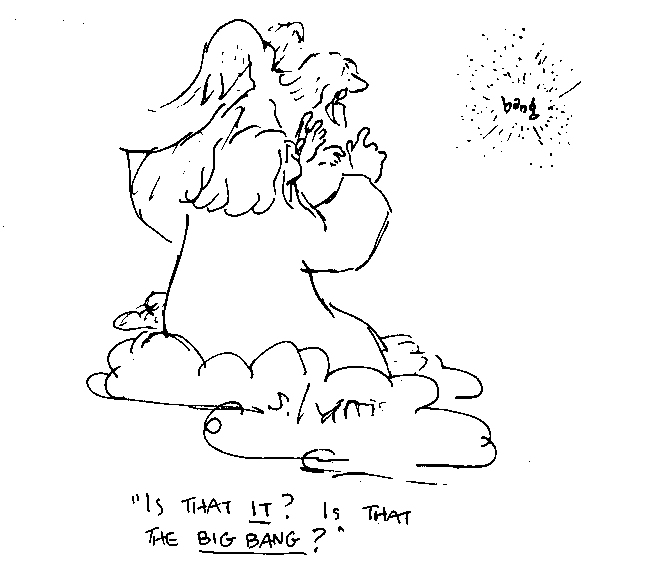
\includegraphics[keepaspectratio,width=12cm]{bang}

\newpage

\begin{itemize}
\item \colorbox{yellow}{Waarom zo "klonterig" verdeeld ?}
\item[] Onderlinge interacties
\item[]\begin{center}{\blue Mechanica (zwaartekracht)}\end{center}
\item \colorbox{yellow}{Wat laat de sterren stralen ?}
\item[] Nucleaire processen
\item[]\begin{center}{\blue Deeltjes fysica}\end{center}
\item \colorbox{yellow}{Emissie en absorbtie lijnen ?}
\item[] Atoom structuur
\item[]\begin{center}{\blue Quantum fysica}\end{center}
\item \colorbox{yellow}{Observatie verschoven spectraallijnen}
\item[] Uitdijend Heelal
\item[]\begin{center}{\blue Kosmologisch model}\end{center}
\end{itemize}

\Transcb{yellow}{blue}{Het onzichtbare heelal}
\onecolumn
\begin{center}
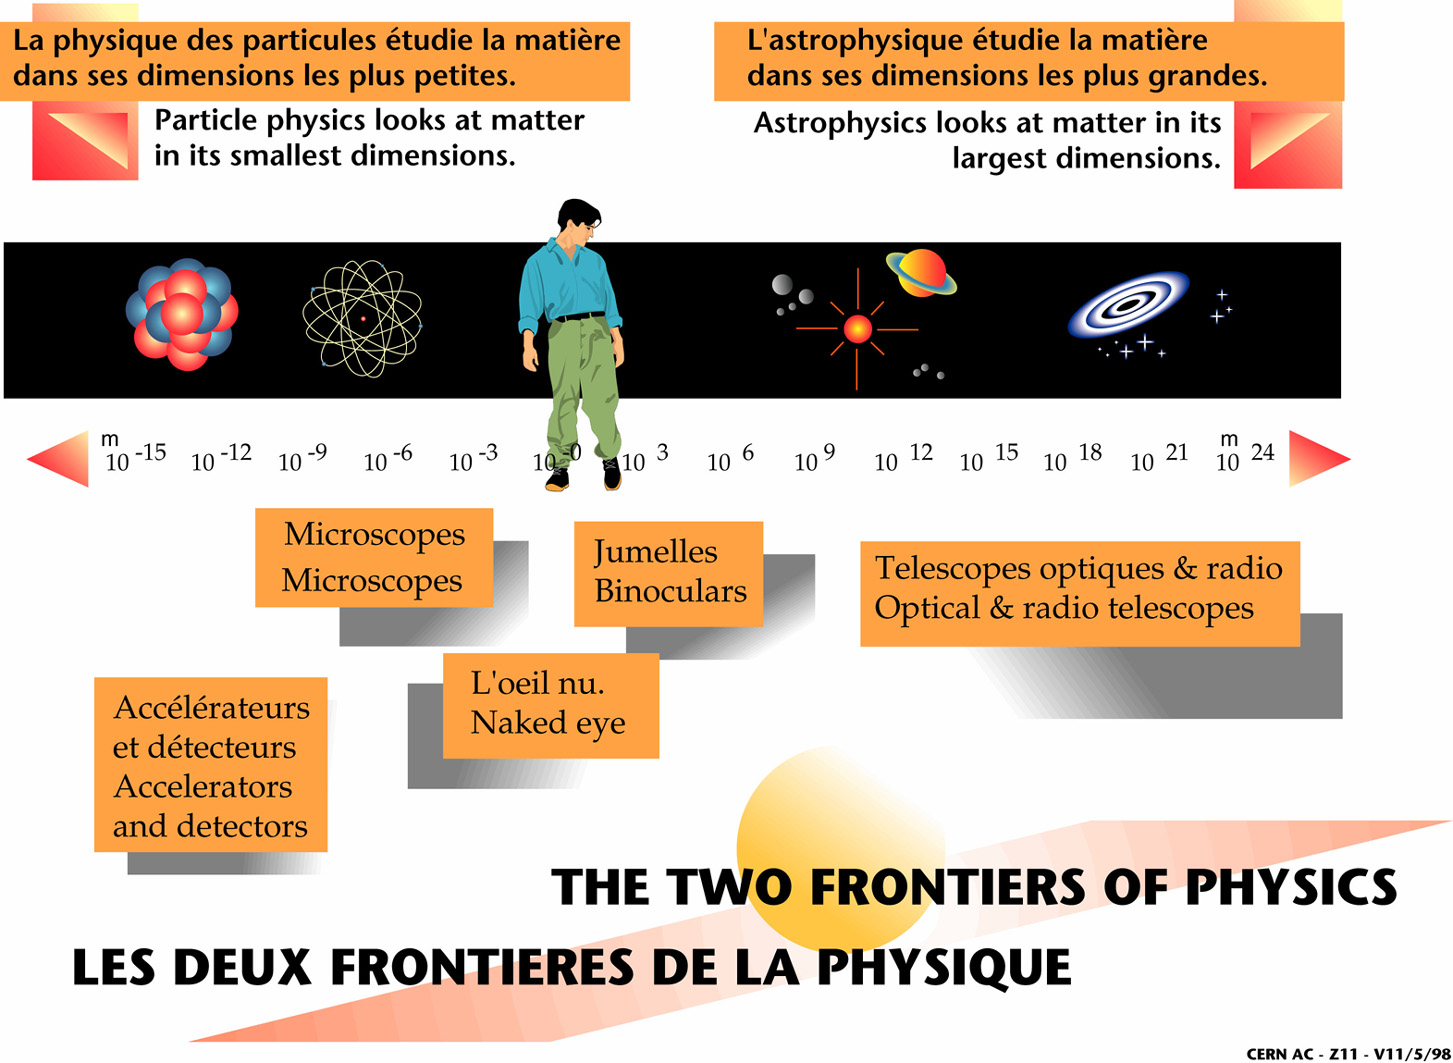
\includegraphics[keepaspectratio,height=14.9cm]{frontiers}
\end{center}

\Tr
\onecolumn
\vspace*{1cm}
\begin{center}
\colorbox{yellow}{Onderzoek naar de structuur van materie}\\[1cm]
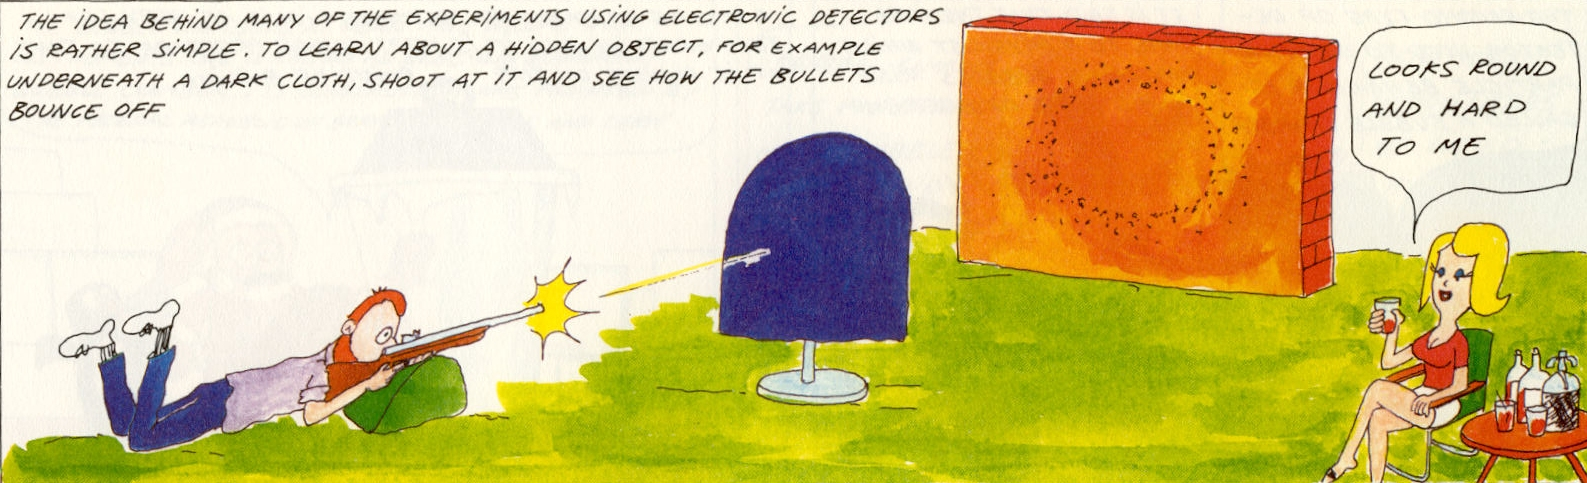
\includegraphics[keepaspectratio,width=25cm]{scatter}
\end{center}

\Tr
\onecolumn
\begin{center}
\colorbox{yellow}{Speurtocht naar nieuwe deeltjes}\\[1cm]
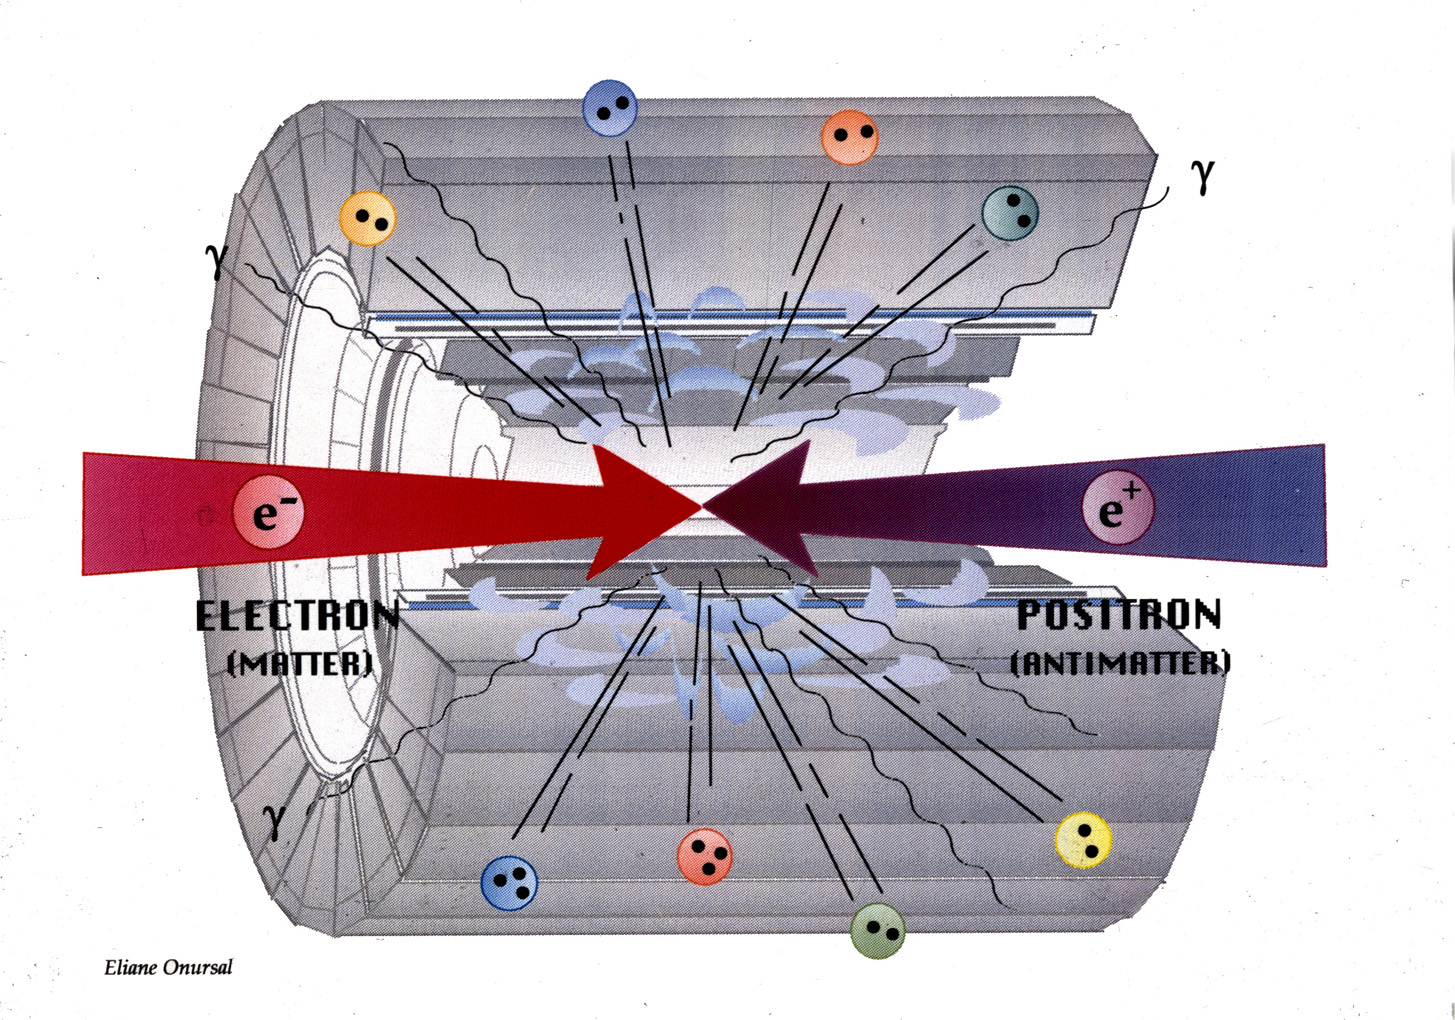
\includegraphics[keepaspectratio,height=12cm]{collision}\\
Deeltjes productie via Energie $-$ Massa conversie ({\blue $E_{rust}=mc^{2}$})
\end{center}

\Tr
\onecolumn
\begin{center}
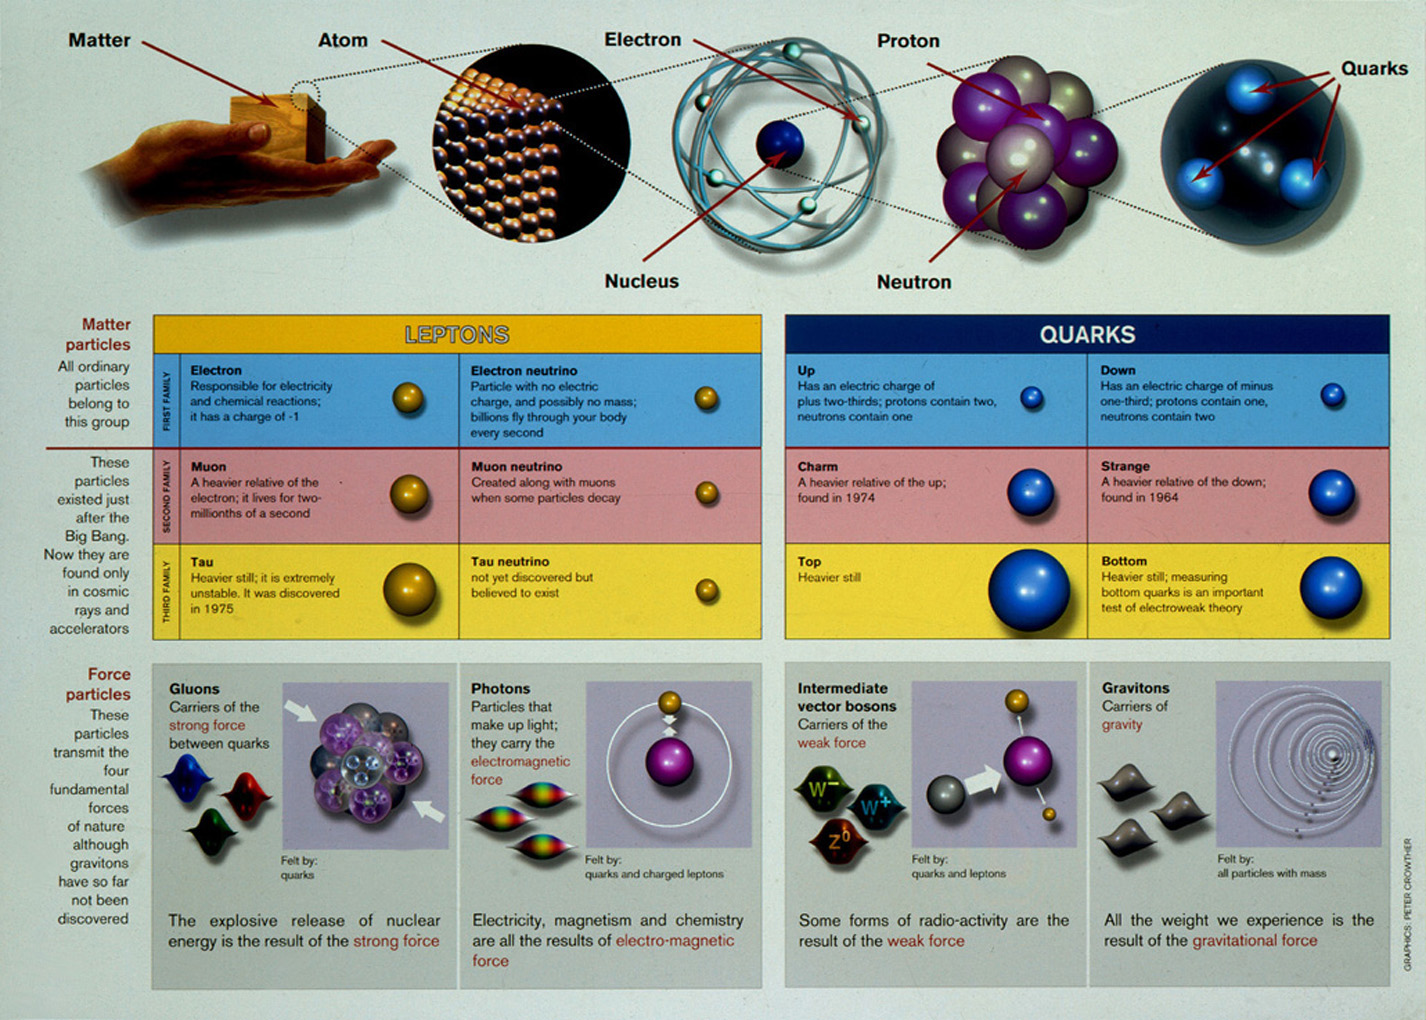
\includegraphics[keepaspectratio,width=20cm]{matter}\\
\colorbox{yellow}{Interacties via uitwisseling van "boodschapper" deeltjes}
\end{center}

\Tr
\twocolumn[\begin{center}\colorbox{yellow}{Kernfusie laat sterren stralen}\end{center}]
%
\begin{center}
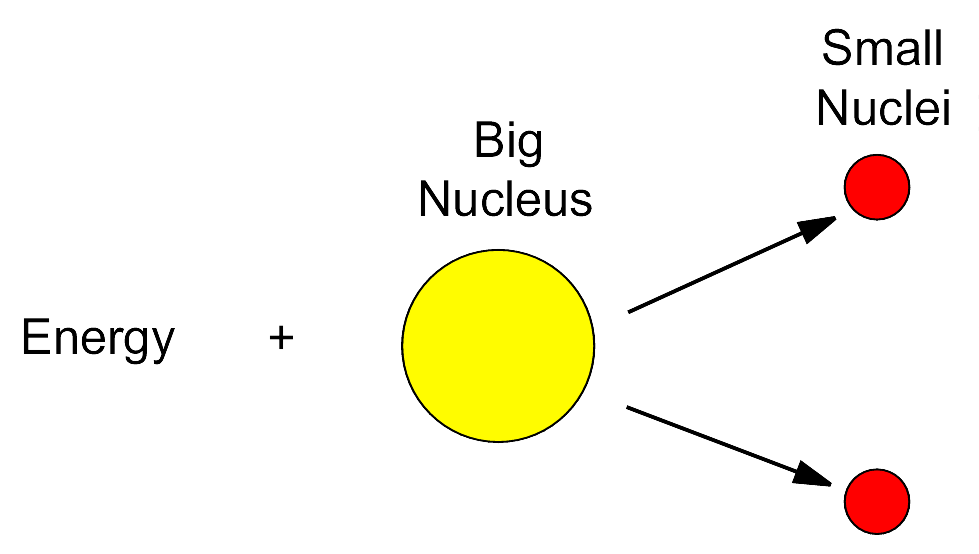
\includegraphics[keepaspectratio,width=10cm]{nuclear-fission}\\[2mm]
{\blue Kernsplitsing}
\end{center}
%
$p+p \rightarrow \Nuc{2}{1}{H}+e^{+}+\nu_{e} \quad \Nuc{2}{1}{H}+p \rightarrow \Nuc{3}{2}{He}+\gamma$ 

\vspace{1cm}

\begin{center}
\colorbox{yellow}{Zwakke kracht produceert neutrinos}\\[2mm]
(Supernovae, AGN, GRBs)
\end{center}
%
\begin{itemize}
\item {\blue Ontstaan van neutronen sterren}
\end{itemize}

\newpage
\begin{center}
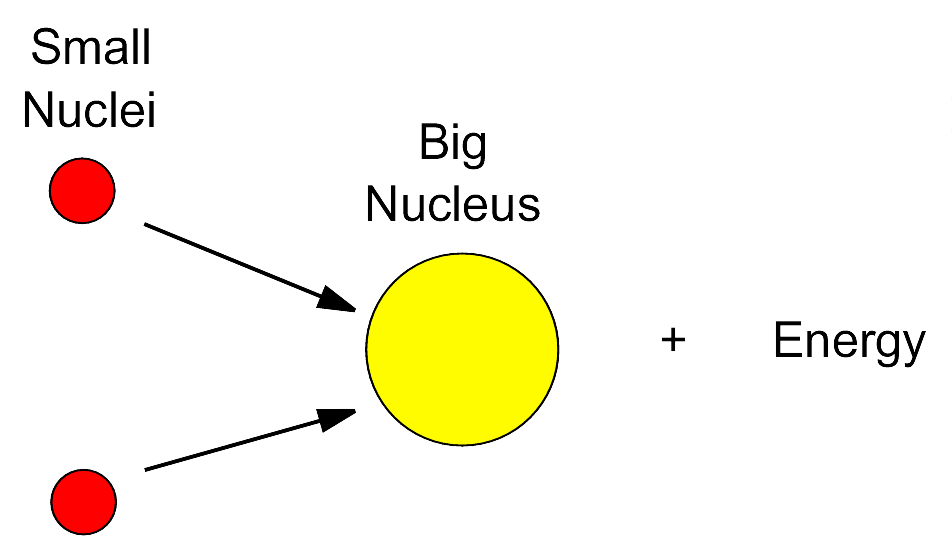
\includegraphics[keepaspectratio,width=10cm]{nuclear-fusion}\\[2mm]
{\blue Kernfusie}
\end{center}
%
$\quad \Nuc{3}{2}{He}+\Nuc{3}{2}{He} \rightarrow \Nuc{4}{2}{He}+p+p$

\vspace{1cm}
\begin{itemize}
\item[] $n \rightarrow p+e^{-}+\bar{\nu}_{e}$
\item[] {\blue $p+e^{-} \rightarrow n+\nu_{e}$}
\item[] $\pi^{-} \rightarrow \mu^{-}+\bar{\nu}_{\mu}$
\item[] $\mu^{-} \rightarrow \nu_{\mu}+e^{-}+\bar{\nu}_{e}$
\end{itemize}

\Tr
\onecolumn
\begin{center}
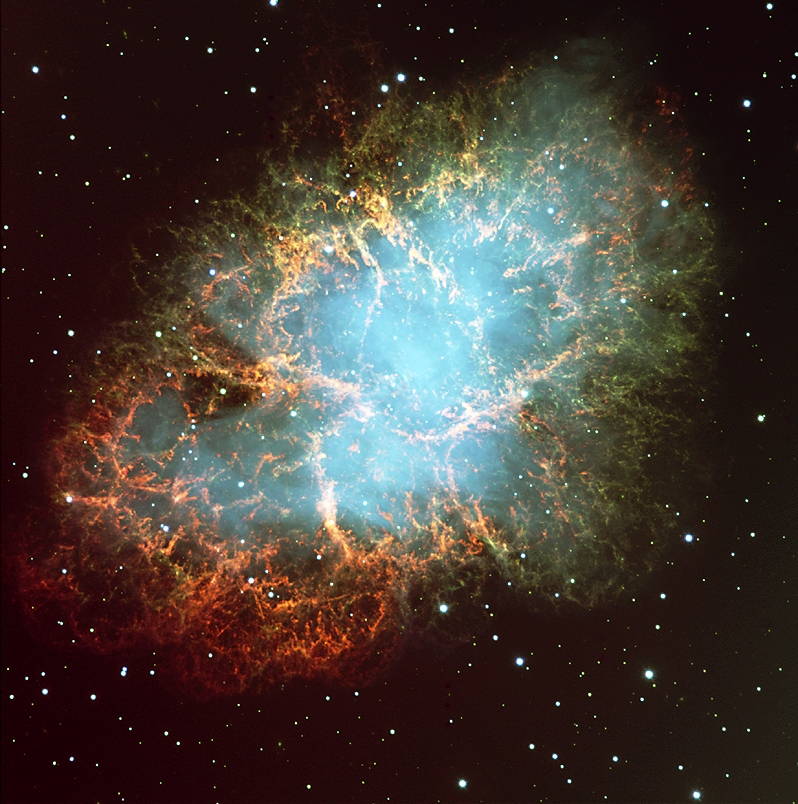
\includegraphics[keepaspectratio,height=15cm]{crab}
\end{center}

\Tr
\begin{center}
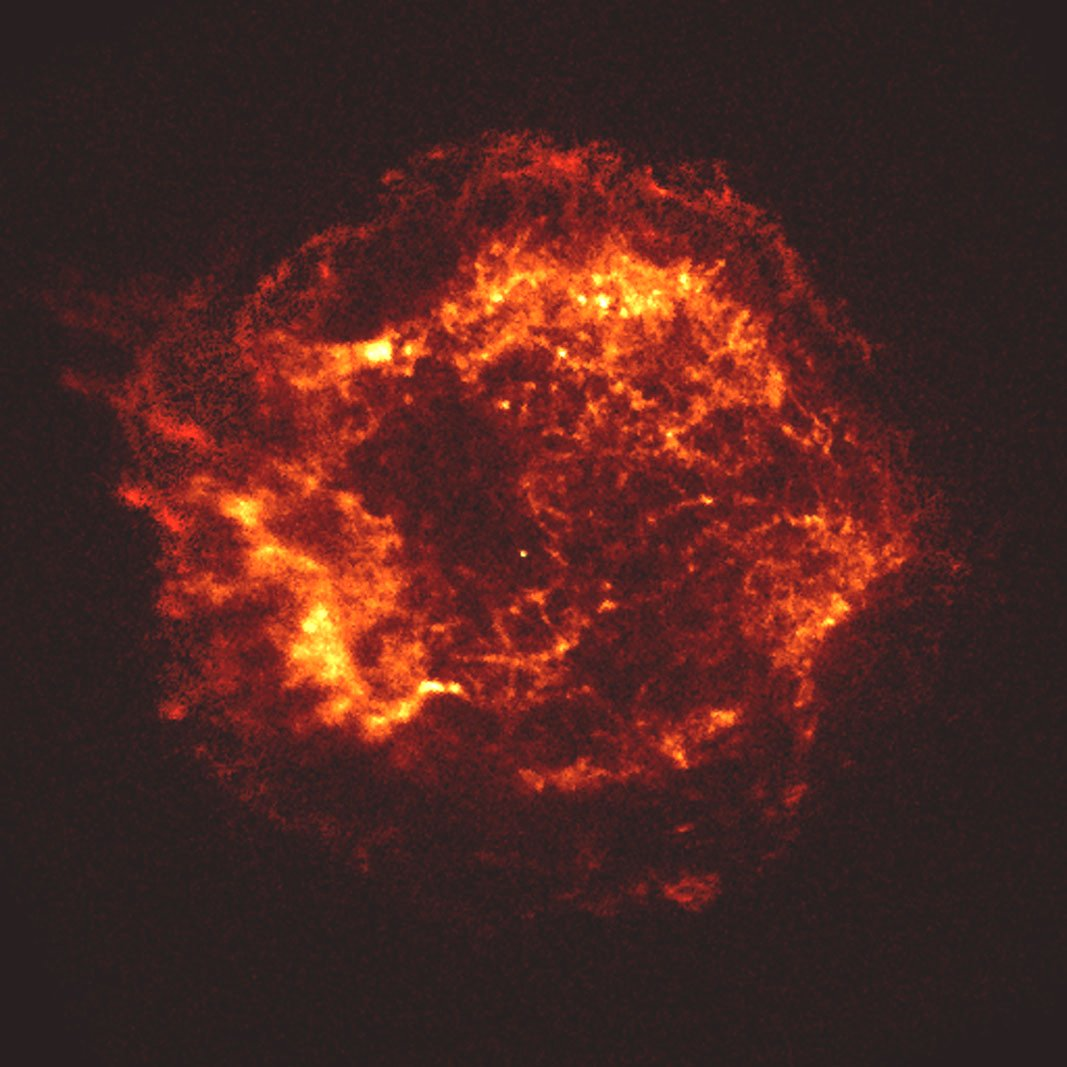
\includegraphics[keepaspectratio,height=15cm]{Cas_A}
\end{center}

\Tr
\twocolumn
\begin{center}
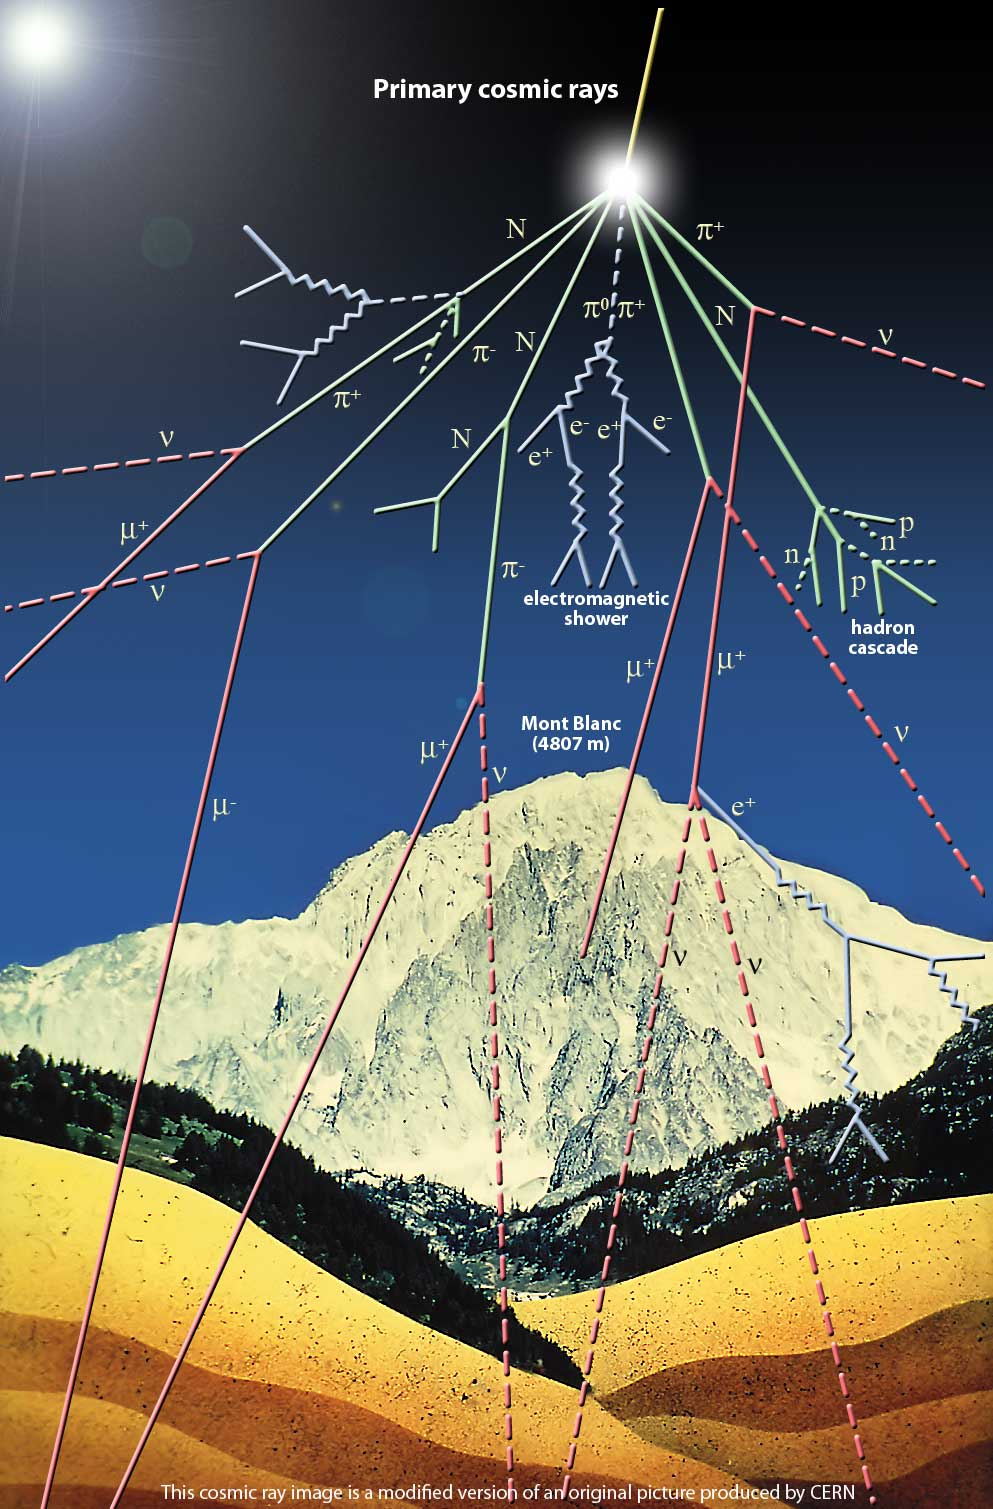
\includegraphics[keepaspectratio,height=15cm]{cosray}
\end{center}

\newpage

\begin{center}
{\blue Spectrum van kosmische straling}\\[5mm]
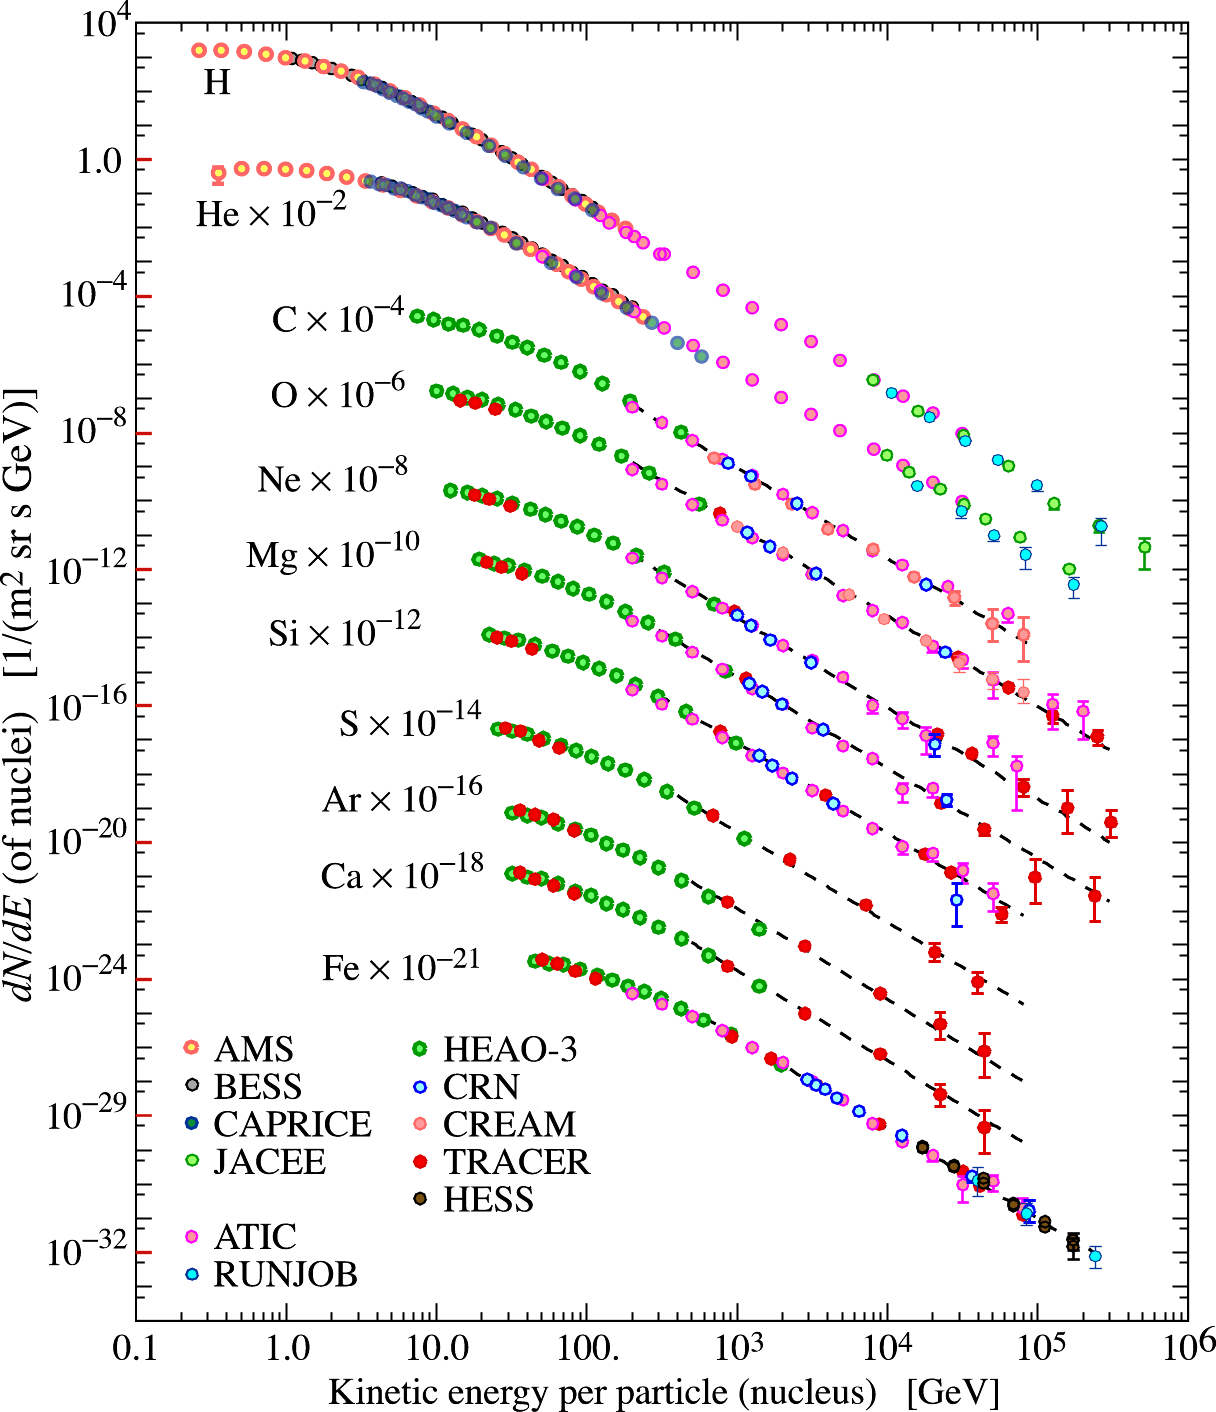
\includegraphics[keepaspectratio,height=14cm]{cr-low-e}
\end{center}

\Tr
\vspace*{1.5cm}
\begin{center}
{\blue $E^{2.6}$ geschaalde flux}\\[5mm]
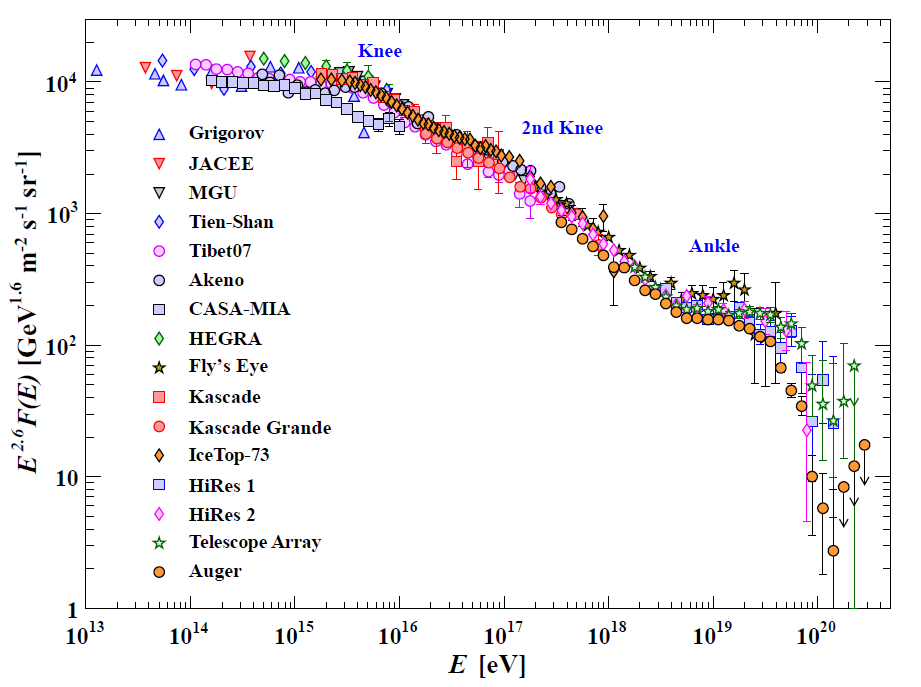
\includegraphics[keepaspectratio,width=13cm]{cr-all-scaled26}
\end{center}

\newpage

\vspace*{3cm}
\begin{itemize}
\item Spectraal structuur (knie, enkel)
\item[] Energetische limieten van kosmische versnellers~?
\item Wat zijn dit voor versnellers~?
\item[] Heftige explosieve fenomenen
\begin{itemize}
\item Supernova's
\item Gammaflitsen
\item Zwarte gaten
\end{itemize}
\end{itemize}

\Tr
\begin{itemize}
\item Supernova schokgolven
\item[] Bewegende lading in mag. veld
\item[] Gyroradius $r=\frac{p}{ZeB} \quad (\vec{p} \perp \vec{B})$
\item[] $\rightarrow
         \left(\frac{p}{1~\rm{eV}}\right)=0.03 \cdot Z\left(\frac{B}{1~\mu\rm{G}}\right)
         \left(\frac{r}{1~\rm{m}}\right)$
\item Versneller van afmeting $R$
\item[] $r > R \rightarrow \text{deeltje~ontsnapt} \rightarrow E_{max}$
\item[] Typisch~: $B \approx \mu\text{G} \quad R \approx 3 \cdot 10^{16}$ m
\item[] $\rightarrow$ Protonen~: $E_{max} \approx 10^{15}$ eV
\item[$\ast$] Bij bepaalde $r \rightarrow {\blue E_{Z}=Z E_{proton}}$
\item[$\ast$] $E>10^{19}~\text{eV} \rightarrow r>R_{melkweg}$
\item[] $\Rightarrow$ Extra-galactische oorsprong
\end{itemize}

\newpage
%
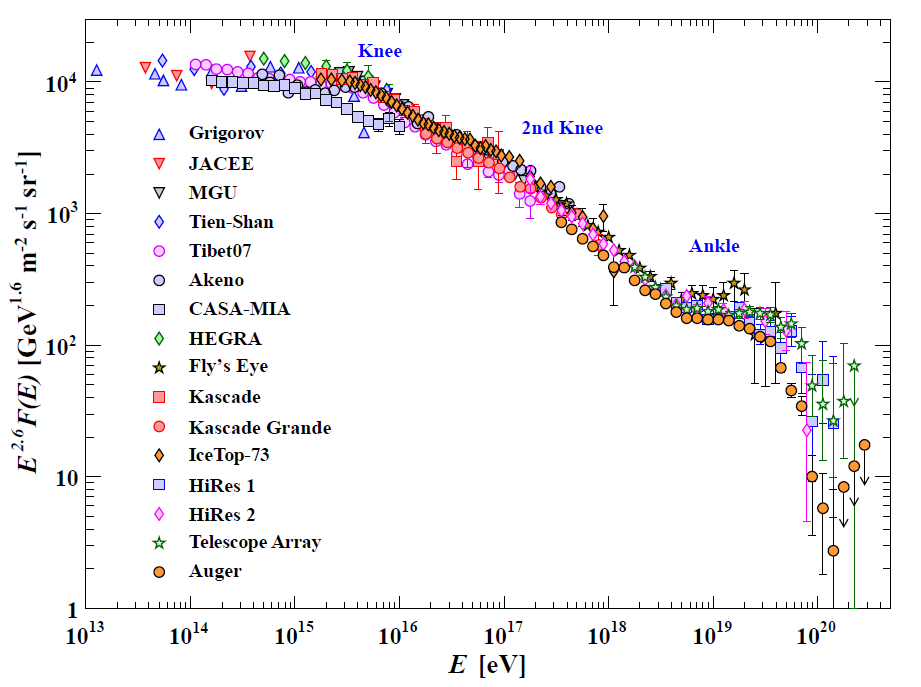
\includegraphics[keepaspectratio,width=13cm]{cr-all-scaled26}
%
\begin{itemize}
\item[] \colorbox{yellow}{Wat veroorzaakt de 'enkel' ?}
\item[] Nog veel krachtiger explosies
\item[] (AGN and GRBs)
\end{itemize}

\Tr
\begin{center}
{\blue Actieve Melkwegkernen (AGN)}\\[1cm]
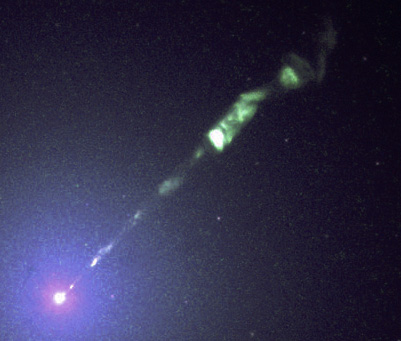
\includegraphics[keepaspectratio,width=13cm]{M87jet}
\end{center}

\newpage

\begin{center}
{\blue Kosmische Gamma Flitsen (GRBs)}\\[1cm]
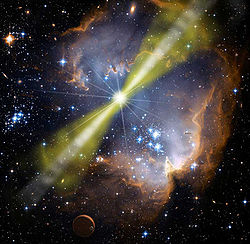
\includegraphics[keepaspectratio,width=6cm]{grb}\\[3mm]
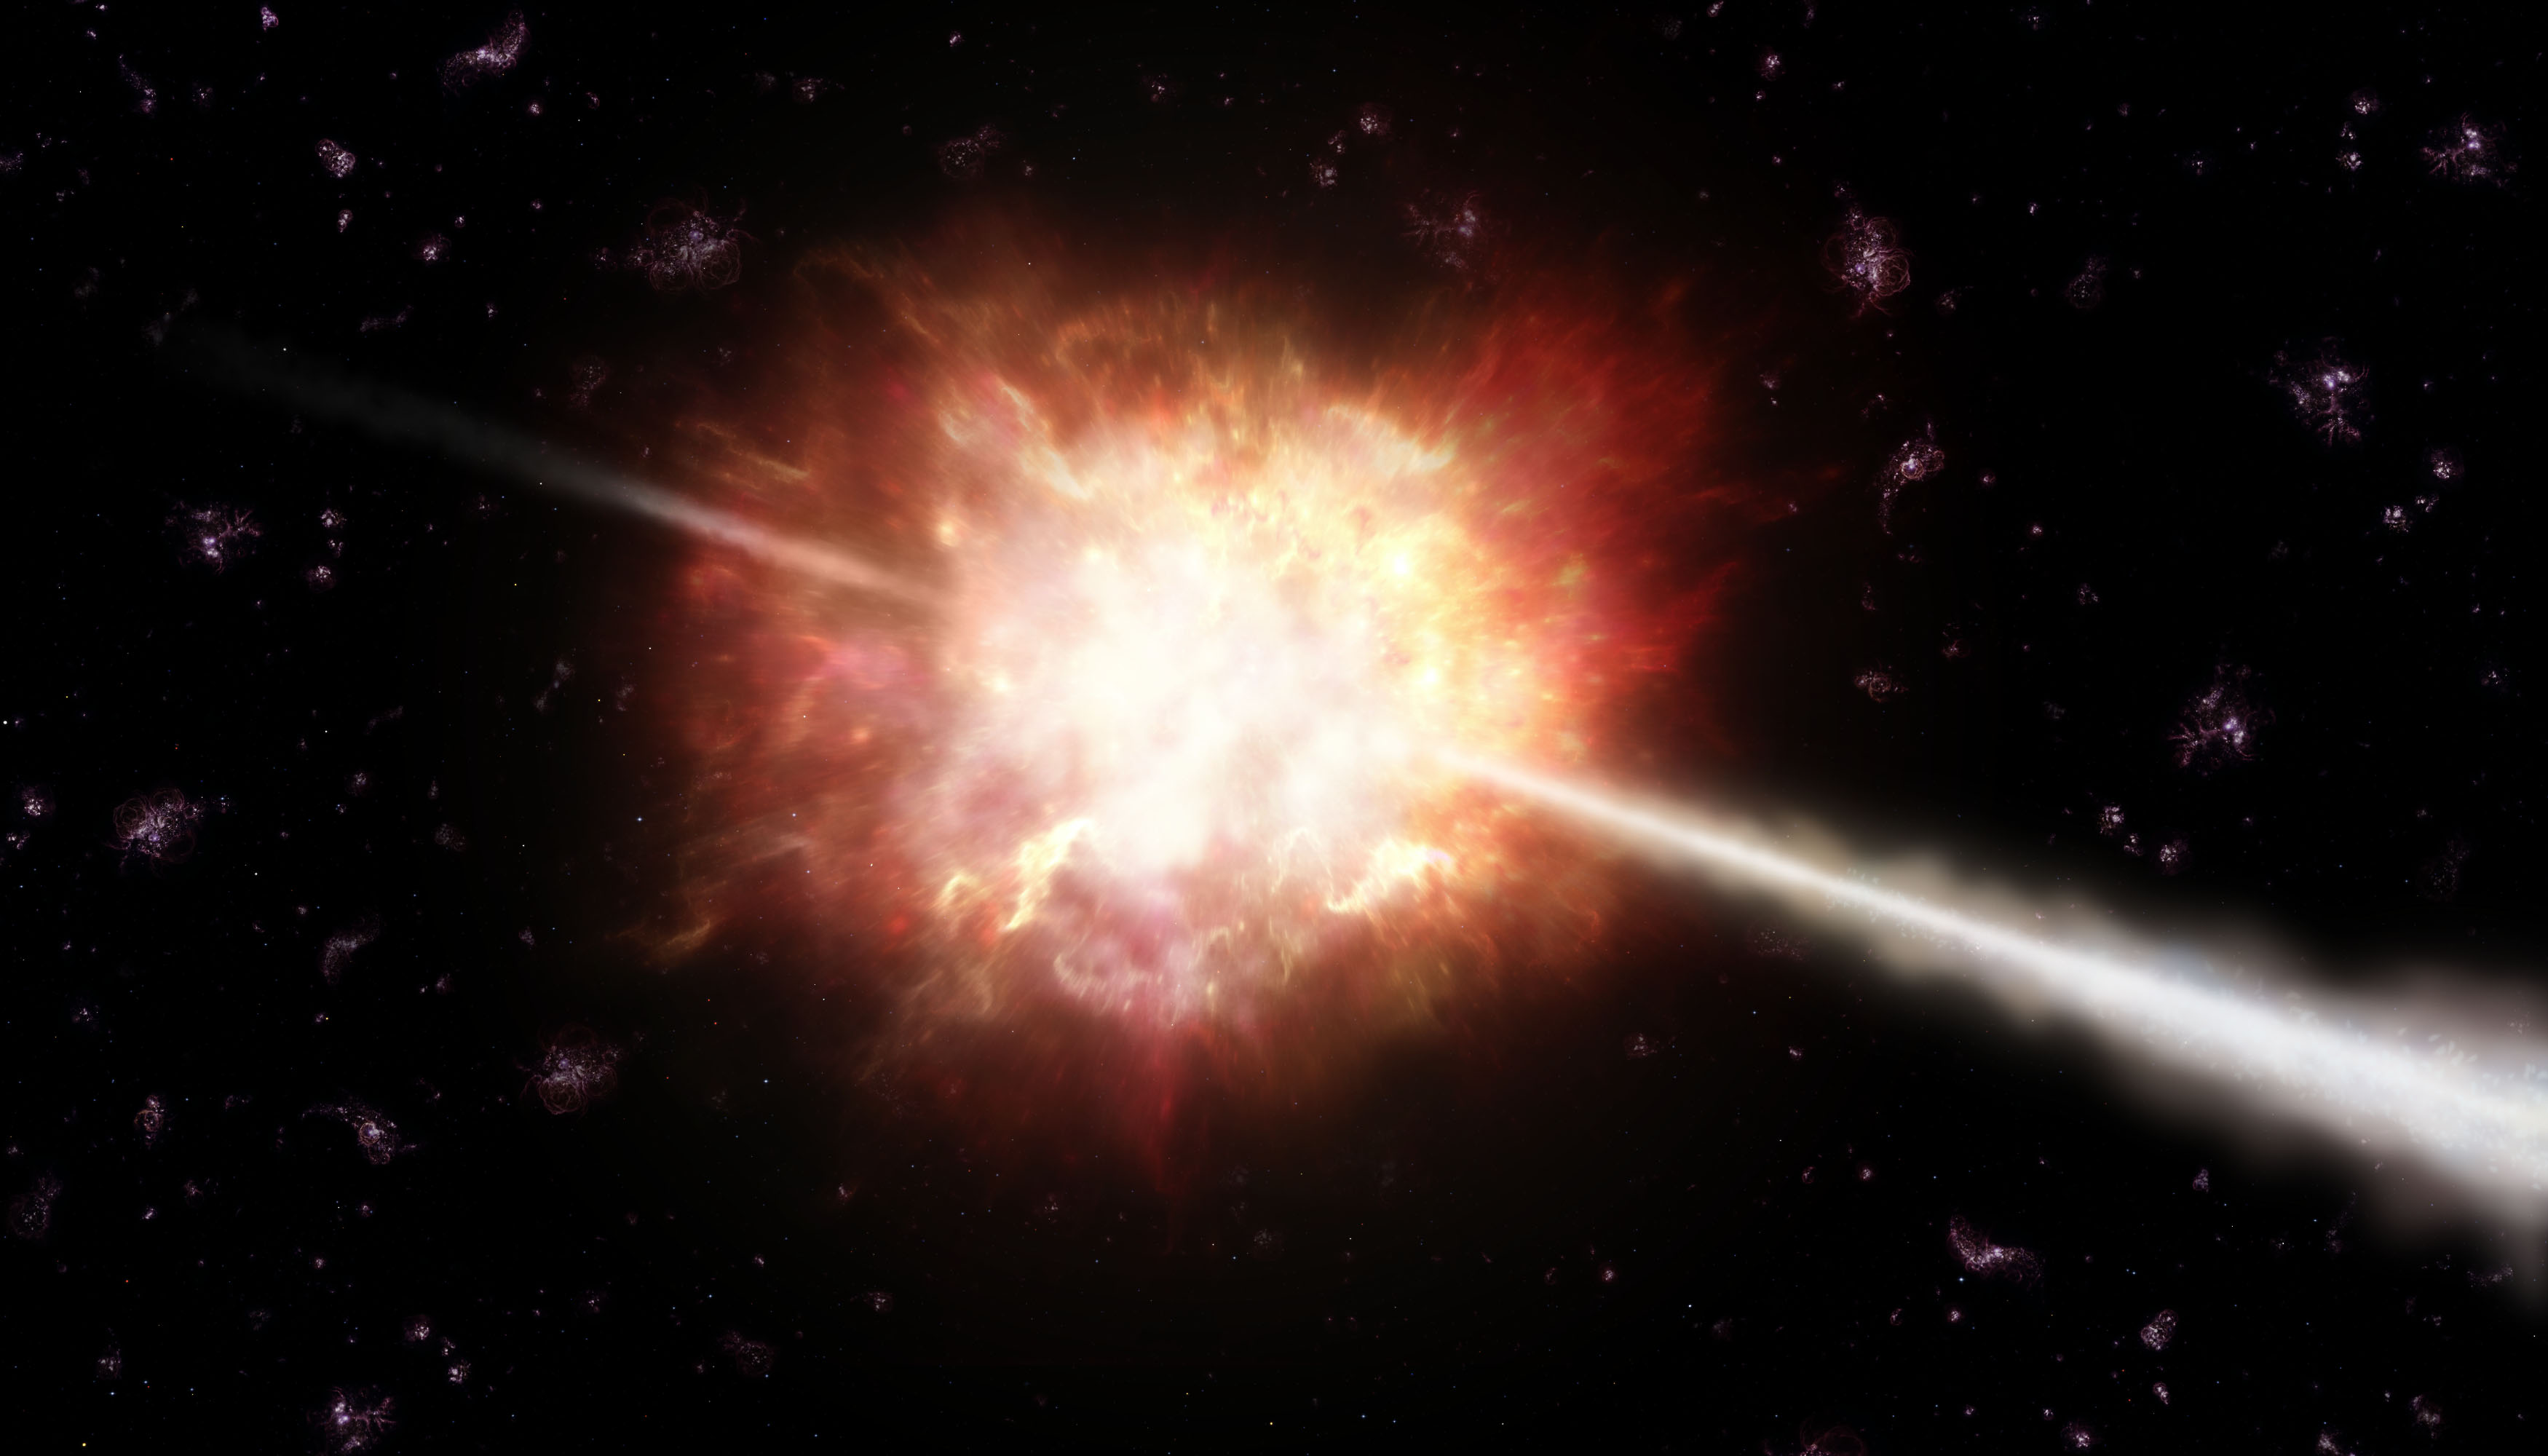
\includegraphics[keepaspectratio,width=12cm]{grb2}
\end{center}

\Tr
\begin{center}
{\blue Algemeen beeld}\\[2mm]
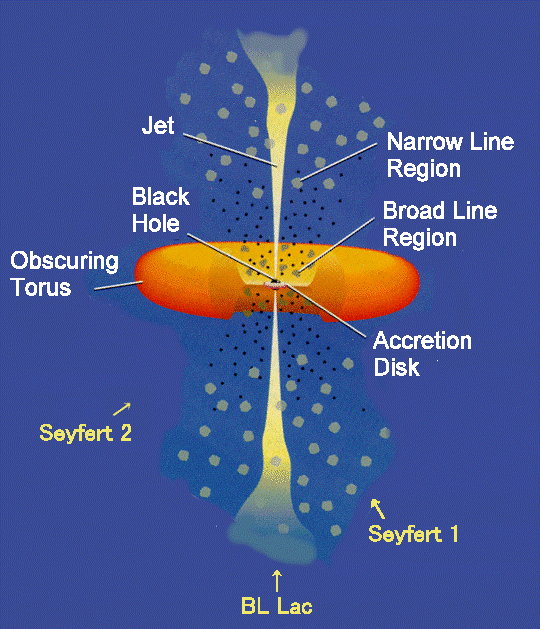
\includegraphics[keepaspectratio,height=12.5cm]{agn-1}\\[5mm]
\colorbox{yellow}{Versnelling in schokgolven}
\end{center}

\newpage

\begin{center}
{\blue Fysische processen}\\[5mm]
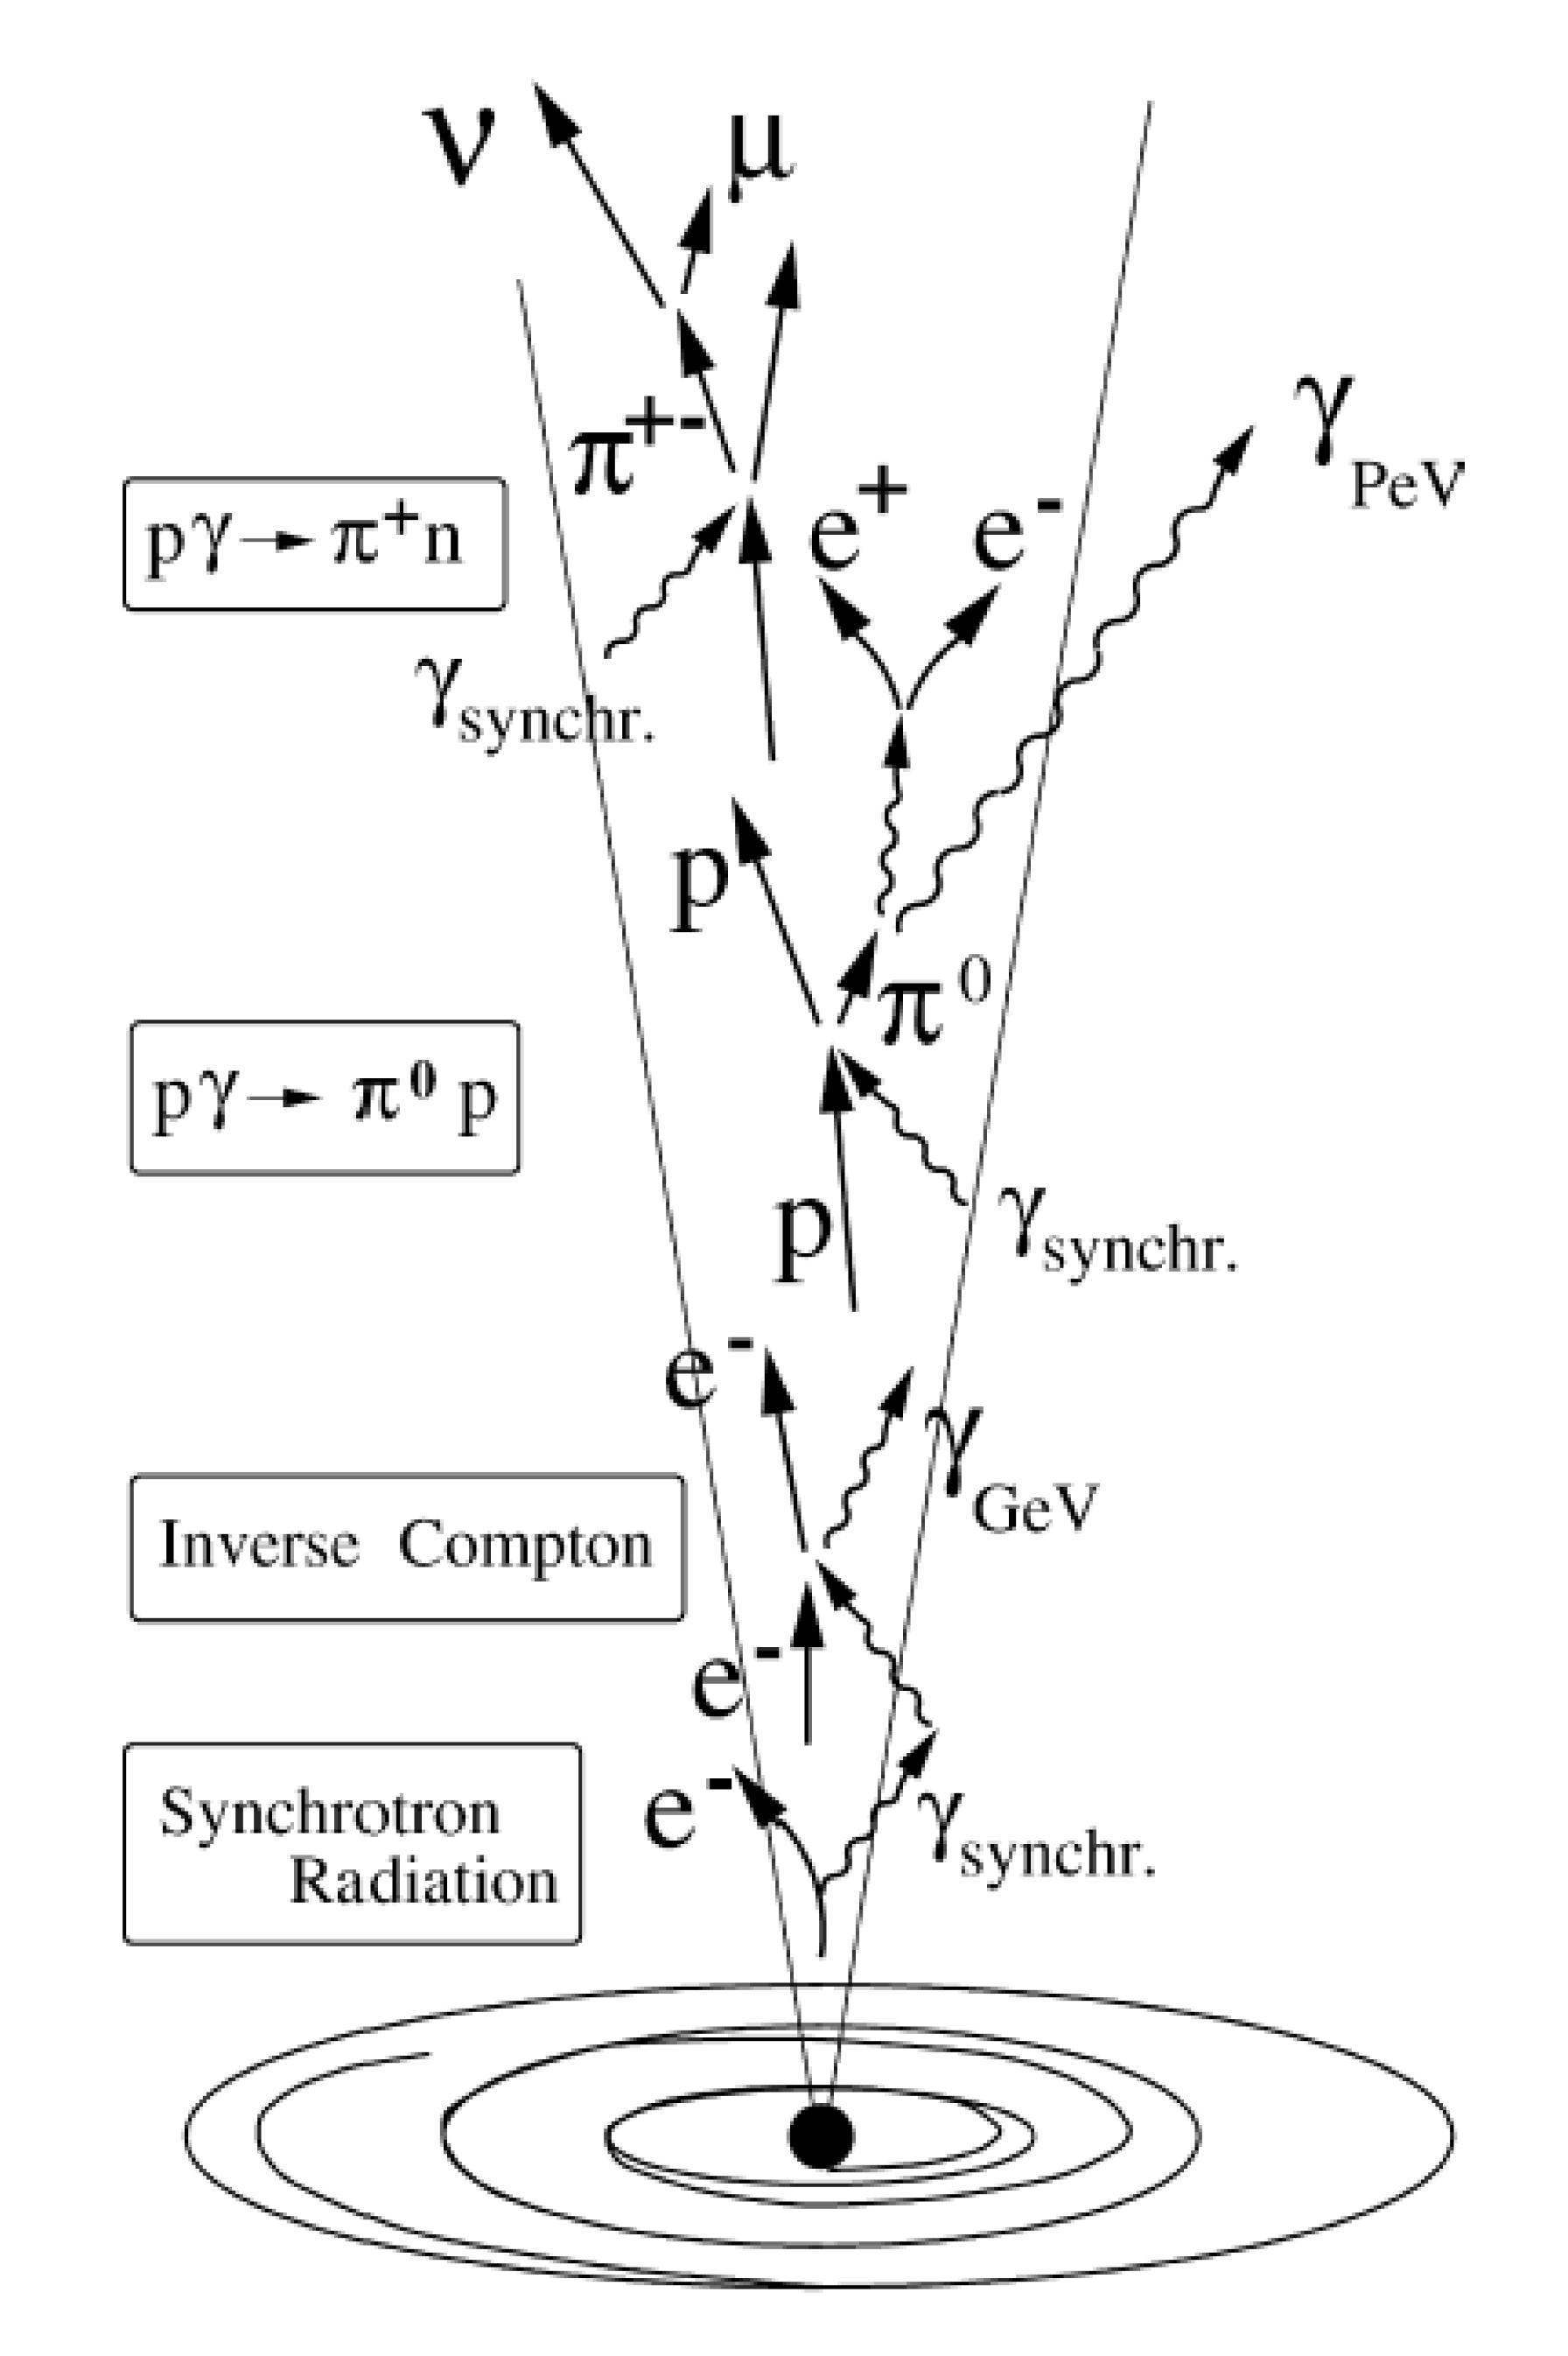
\includegraphics[keepaspectratio,height=12.3cm]{jet}\\[5mm]
\colorbox{yellow}{Hoog-energetische fotonen en neutrinos}
\end{center}

\Transcb{yellow}{blue}{Jacht op kosmische neutrinos}
\twocolumn
\begin{center}
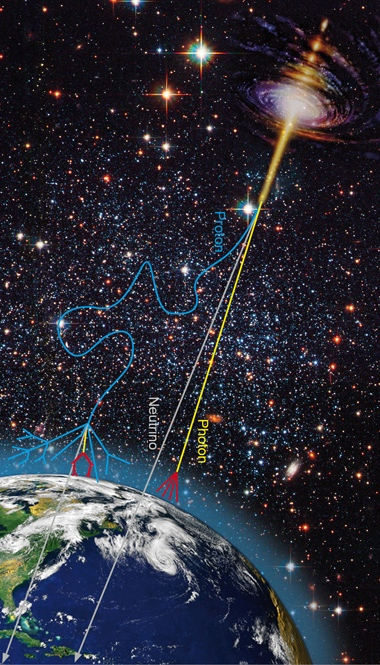
\includegraphics[keepaspectratio,height=15.7cm]{app-vertical}
\end{center}

\newpage
\begin{center}
{\blue Neutrino detectie mechanisme}\\[5mm]
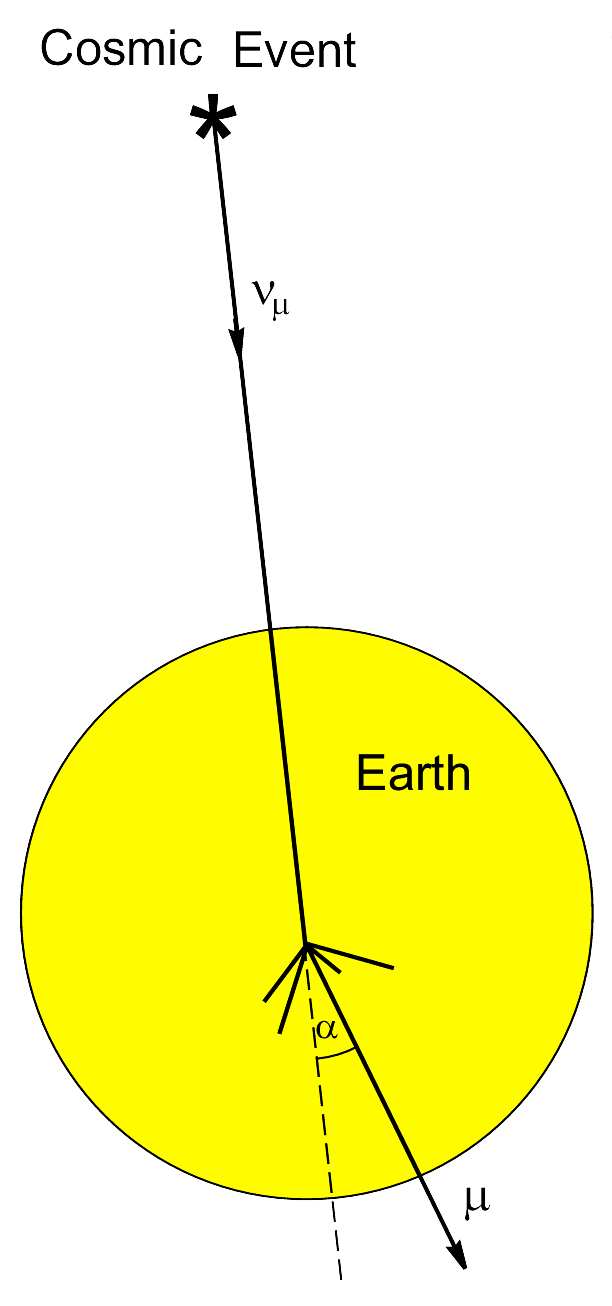
\includegraphics[keepaspectratio,height=14cm]{earth-shield}
\end{center}

\Transcb{yellow}{blue}{De IceCube Neutrino Telescoop}
\onecolumn
\begin{center}
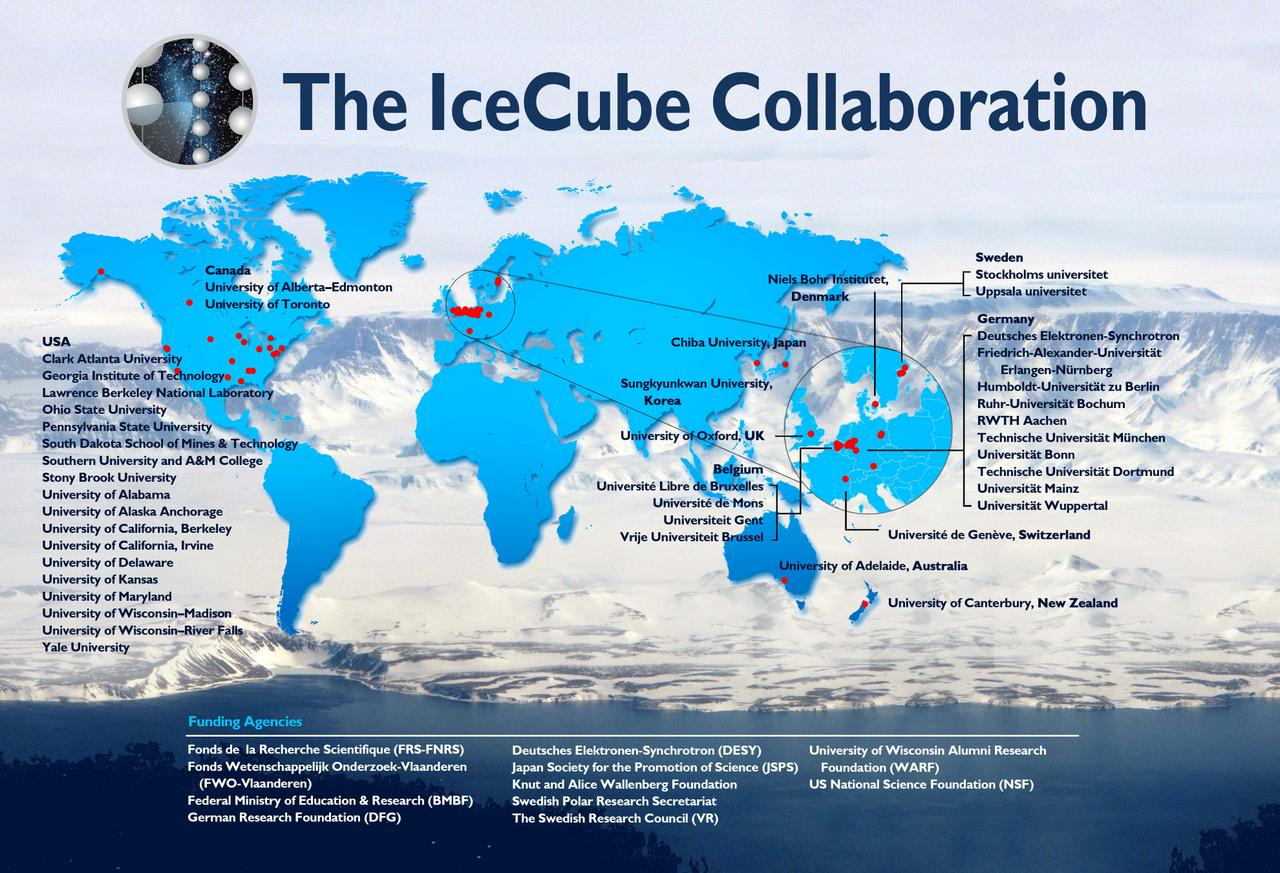
\includegraphics[keepaspectratio,height=15cm]{icecube-collab}
\end{center}

\Tr
\begin{center}
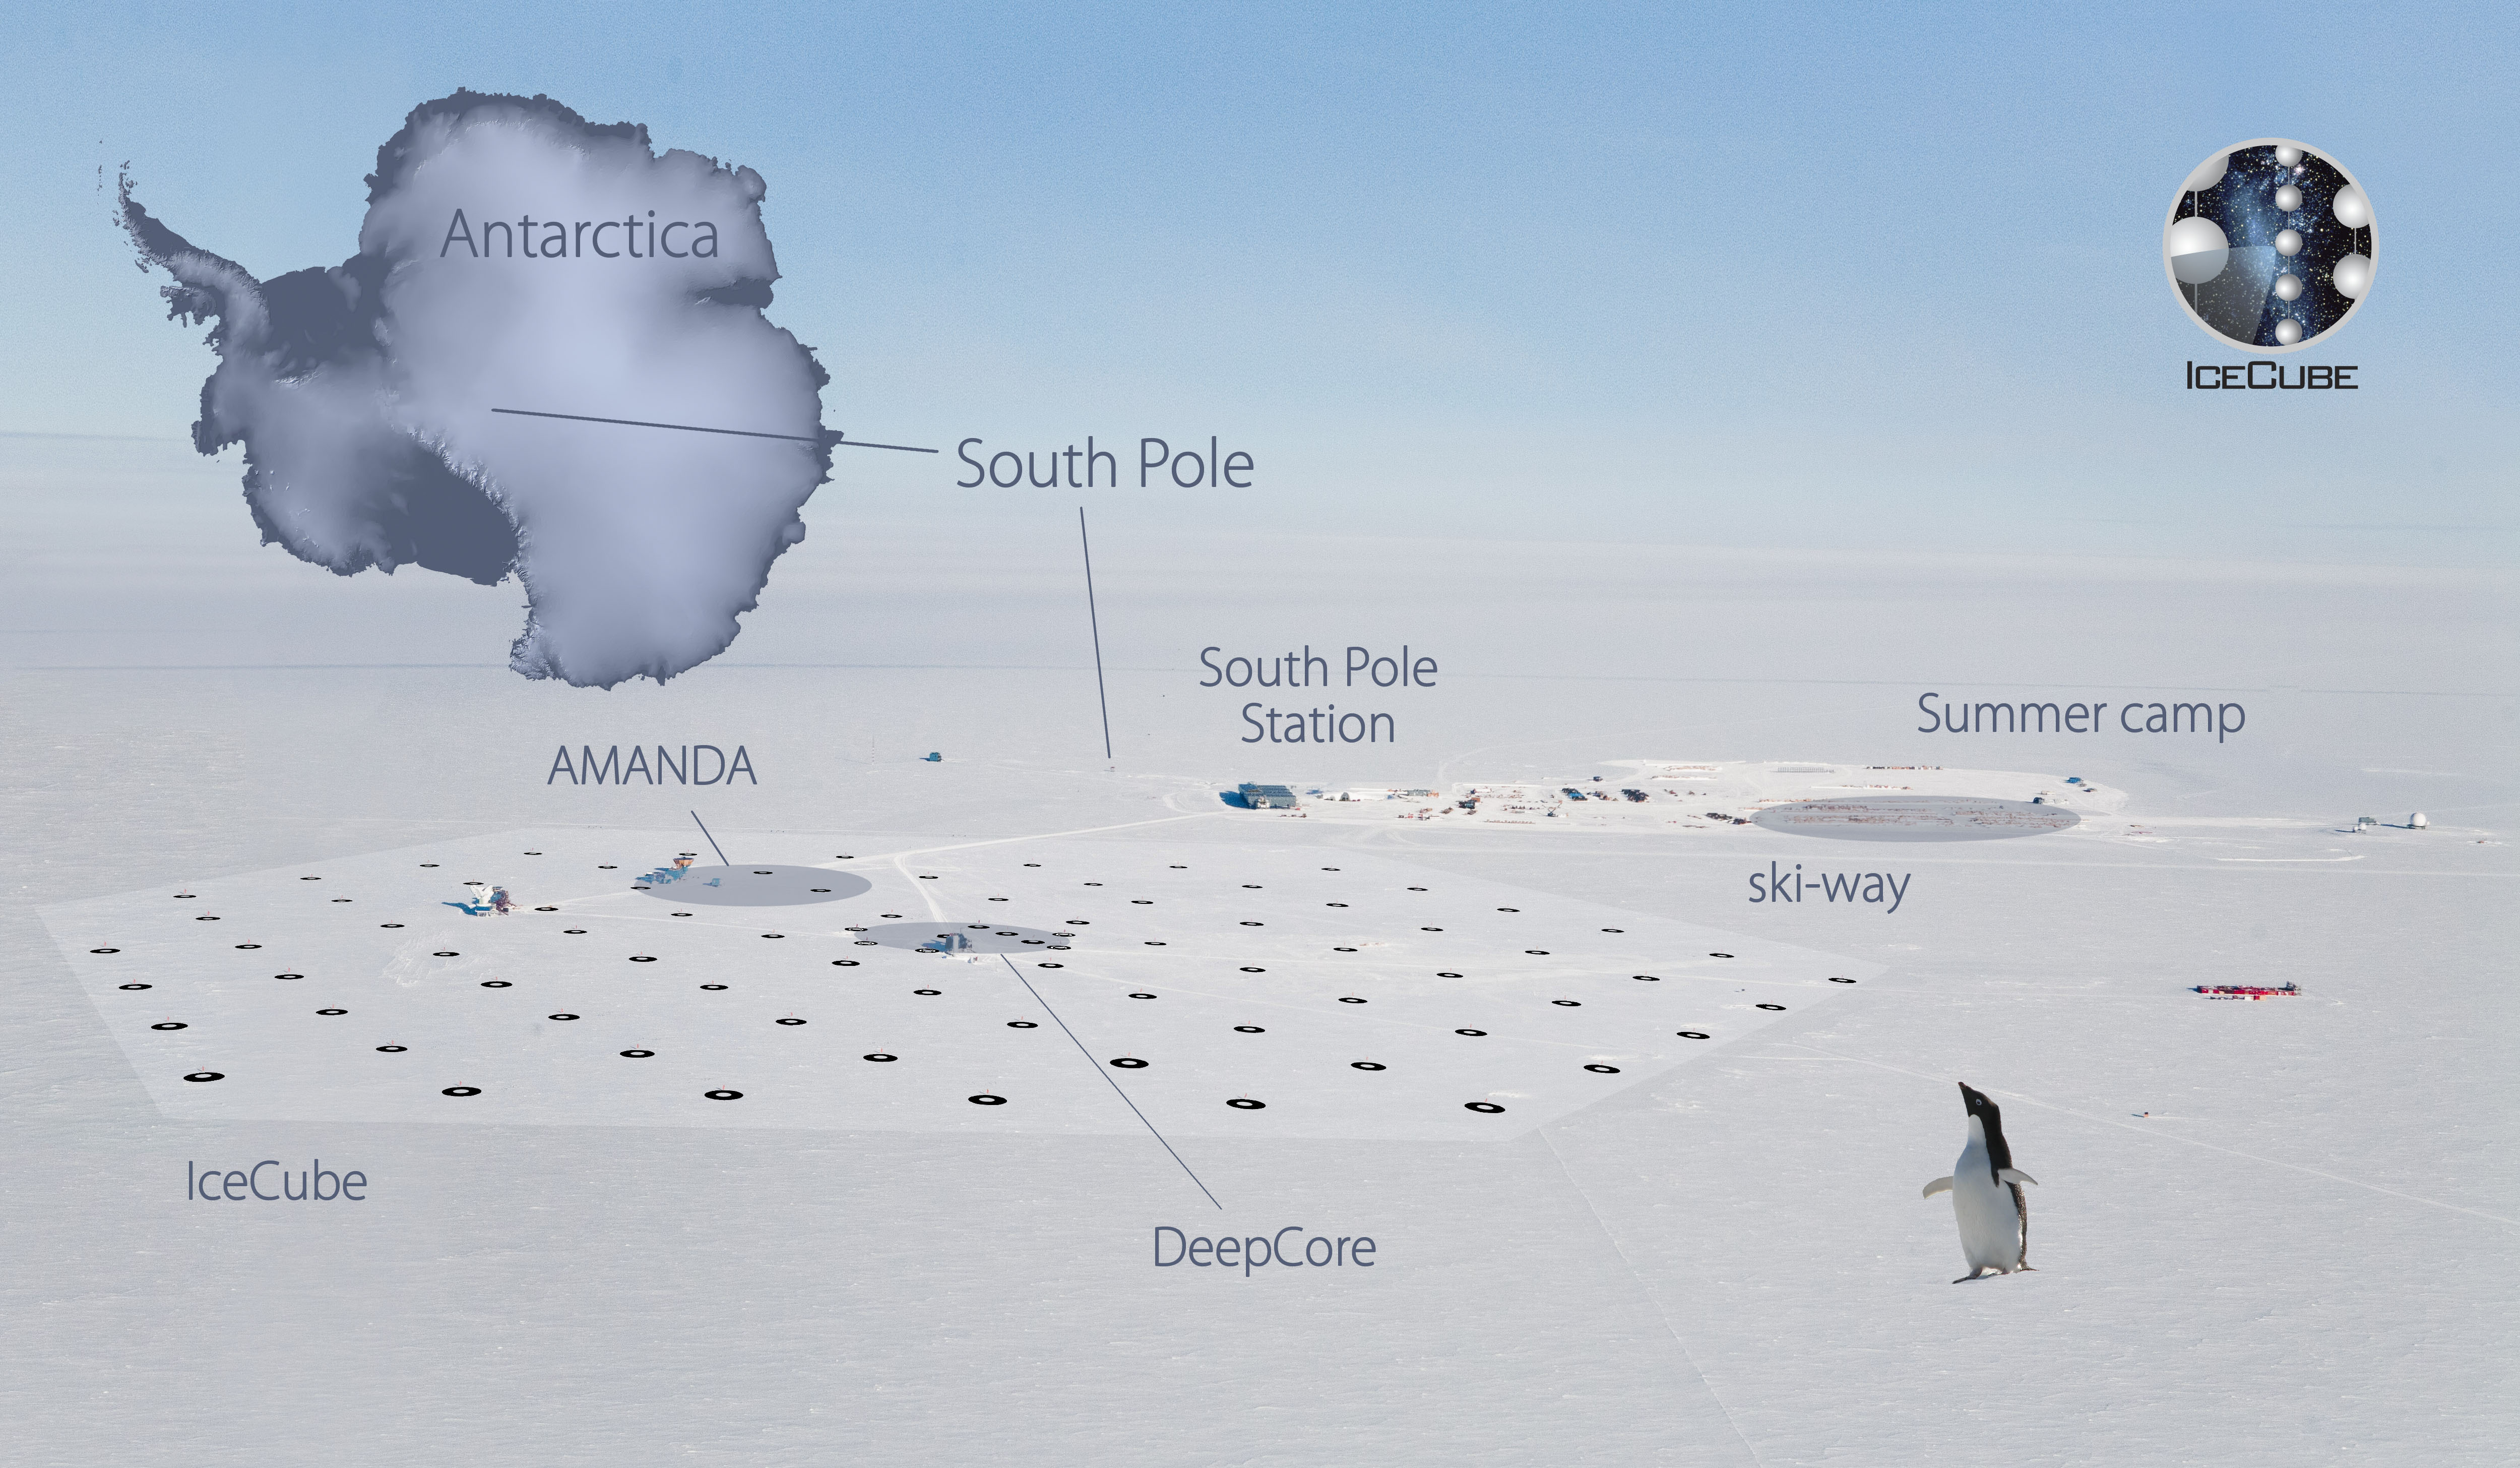
\includegraphics[keepaspectratio,height=14.5cm]{pole-view}
\end{center}

\Tr
\vspace*{1cm}
\begin{center}
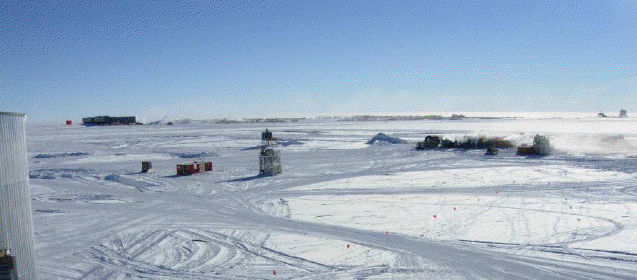
\includegraphics[keepaspectratio,width=25cm]{camp-view}
\end{center}

\Tr
\begin{center}
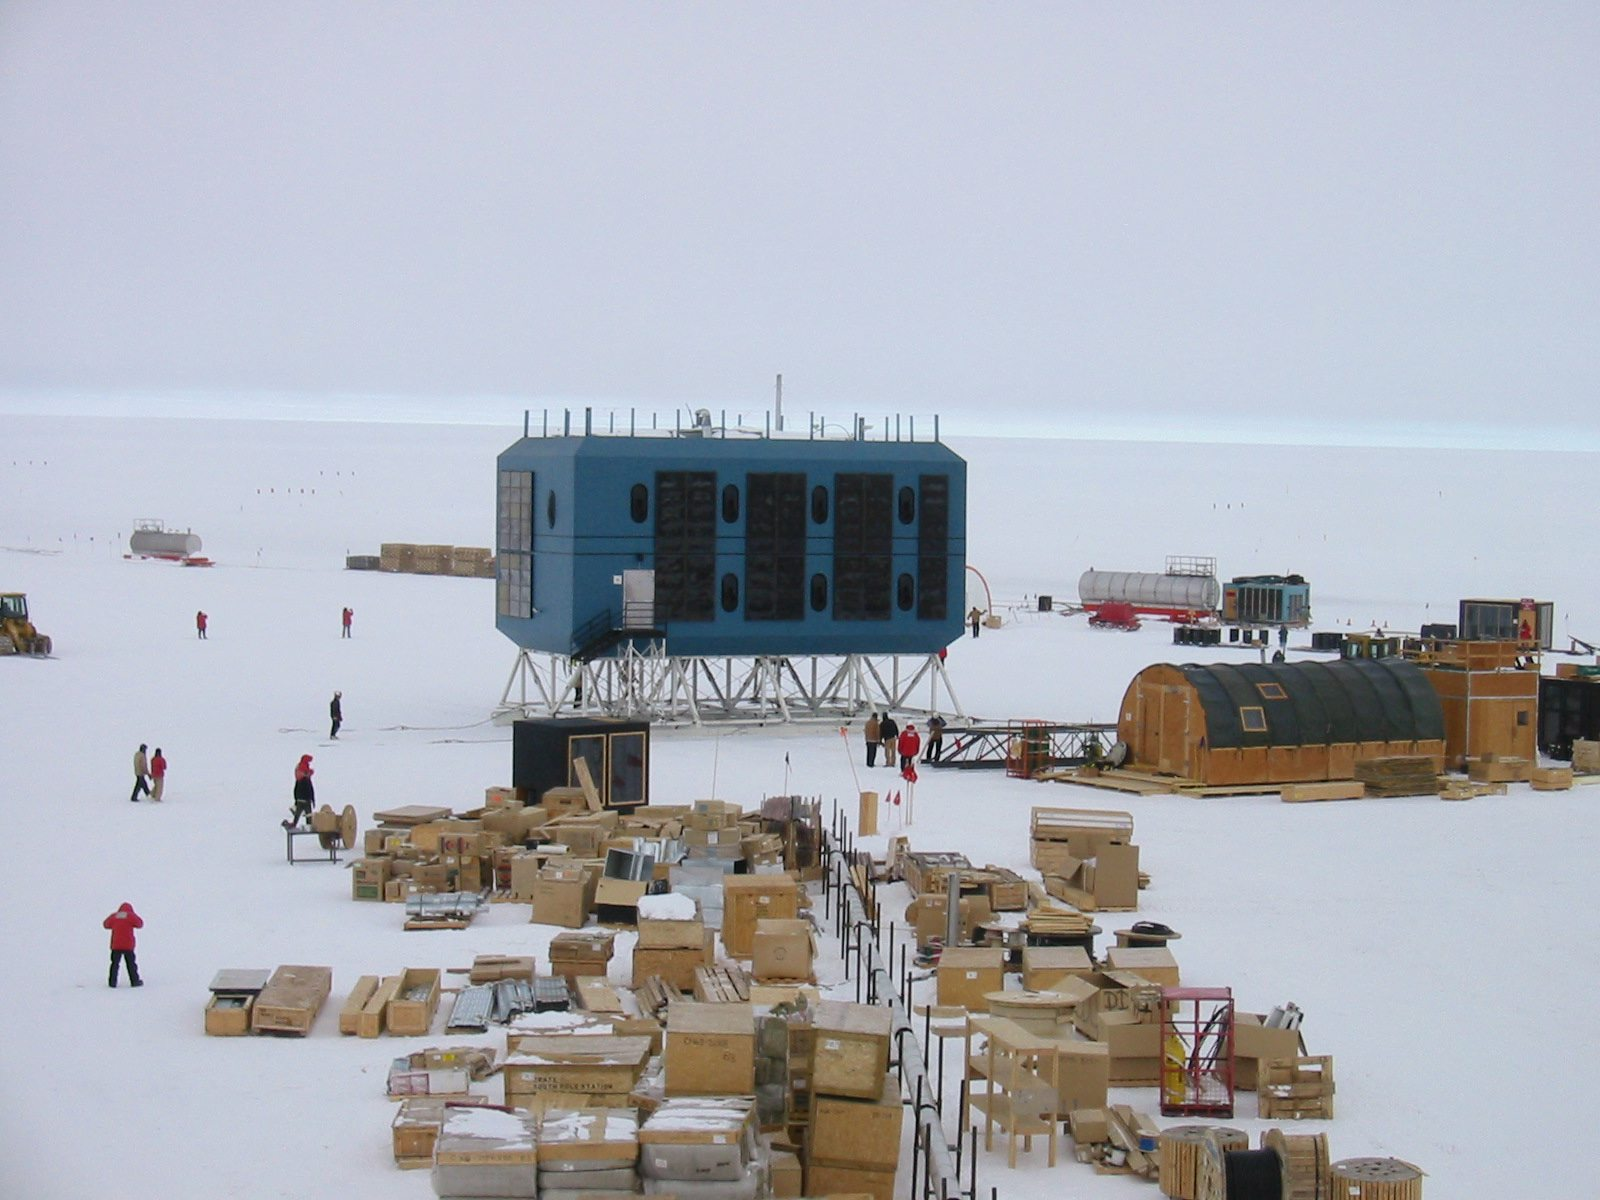
\includegraphics[keepaspectratio,height=14.5cm]{counting-house}
\end{center}

\Tr
\begin{center}
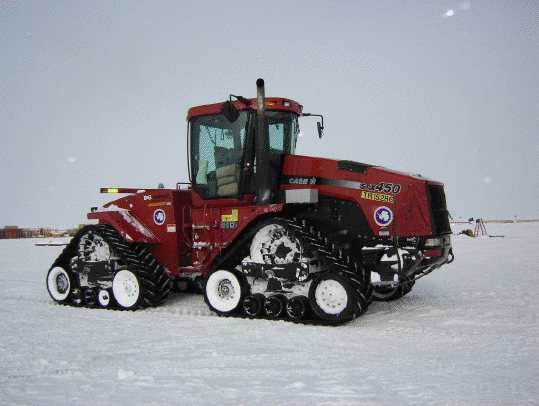
\includegraphics[keepaspectratio,height=14.5cm]{tractor}
\end{center}

\Tr
\begin{center}
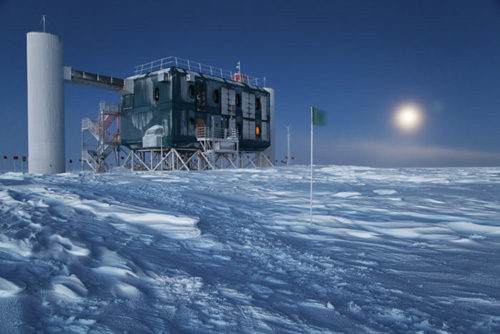
\includegraphics[keepaspectratio,height=14cm]{icl2}
\end{center}

\Tr
\begin{center}
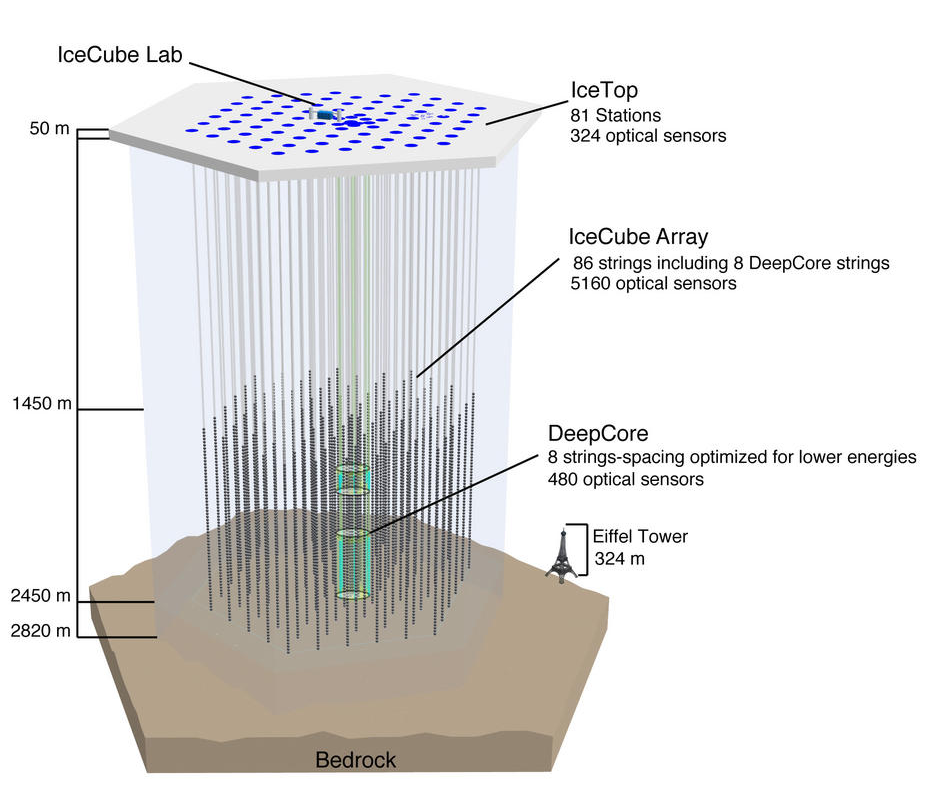
\includegraphics[keepaspectratio,height=14cm]{ic86-dc}
\end{center}

\Tr
\begin{center}
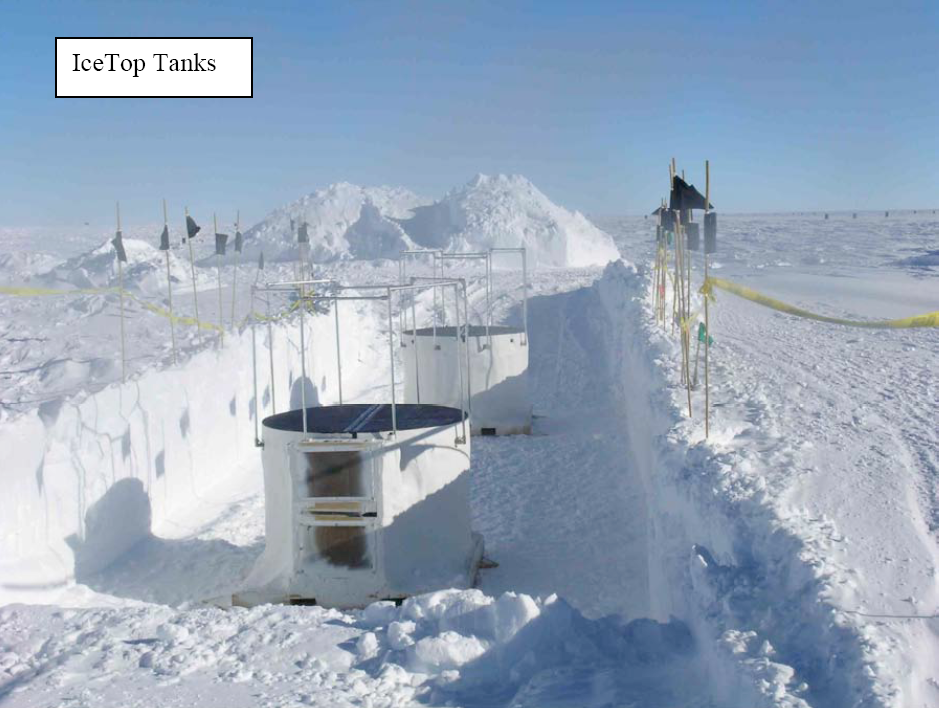
\includegraphics[keepaspectratio,height=14.5cm]{icetop-snow}
\end{center}

\Tr
\begin{center}
{\blue IceTop detectie principe}\\[5mm] 
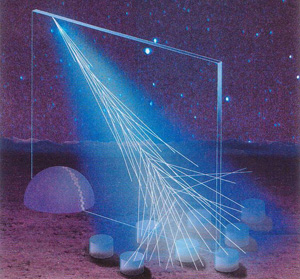
\includegraphics[keepaspectratio,height=14cm]{cr-shower}
\end{center}

\Tr
\begin{center}
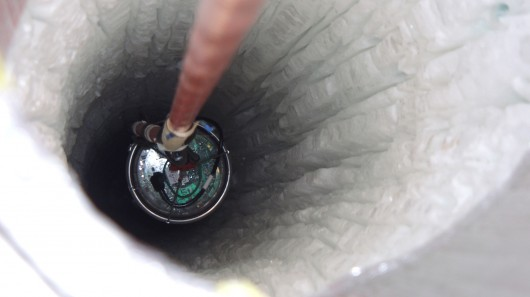
\includegraphics[keepaspectratio,height=14cm]{hole2}
\end{center}

\Tr
\twocolumn[\begin{center}{\blue InIce detectie principe}\end{center}]
\begin{center}
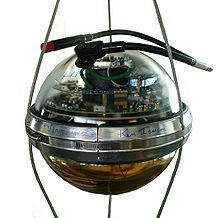
\includegraphics[keepaspectratio,height=6cm]{dom}\\[3mm]
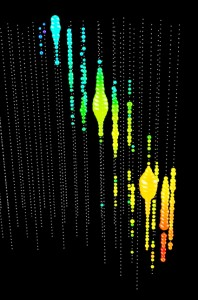
\includegraphics[keepaspectratio,height=7cm]{event}
\end{center}
%
\newpage
%
\begin{center}
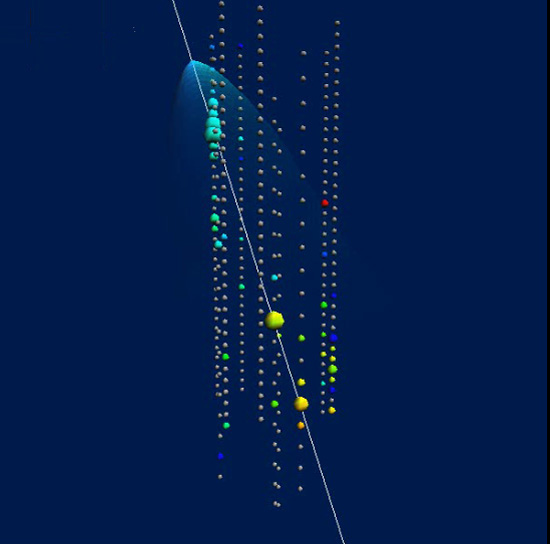
\includegraphics[keepaspectratio,width=13.5cm]{cone}
\end{center}

\Tr
\onecolumn
\begin{center}
{\red Muonen van atmosferische interacties}\\[1cm]
{\blue De schaduw van de Maan}\\[5mm]
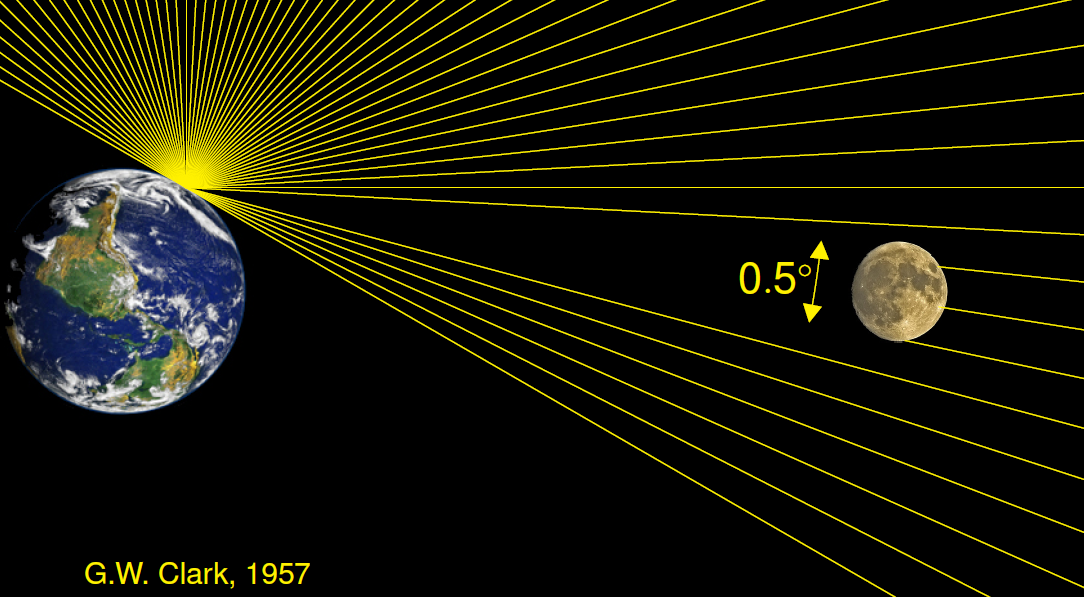
\includegraphics[keepaspectratio,height=8cm]{moon-shadow1}
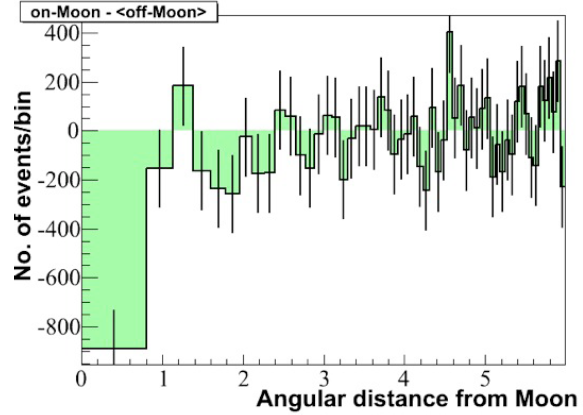
\includegraphics[keepaspectratio,height=8cm]{moon-shadow2}\\[1cm]
{\blue Hoekresolutie : $\sim 0.8^{\circ}$}
\end{center}

\Tr
\onecolumn
\begin{center}
{\blue De IceCube hemelkaart} (7 jaar data, $\sim$700'000 events)\\[5mm]
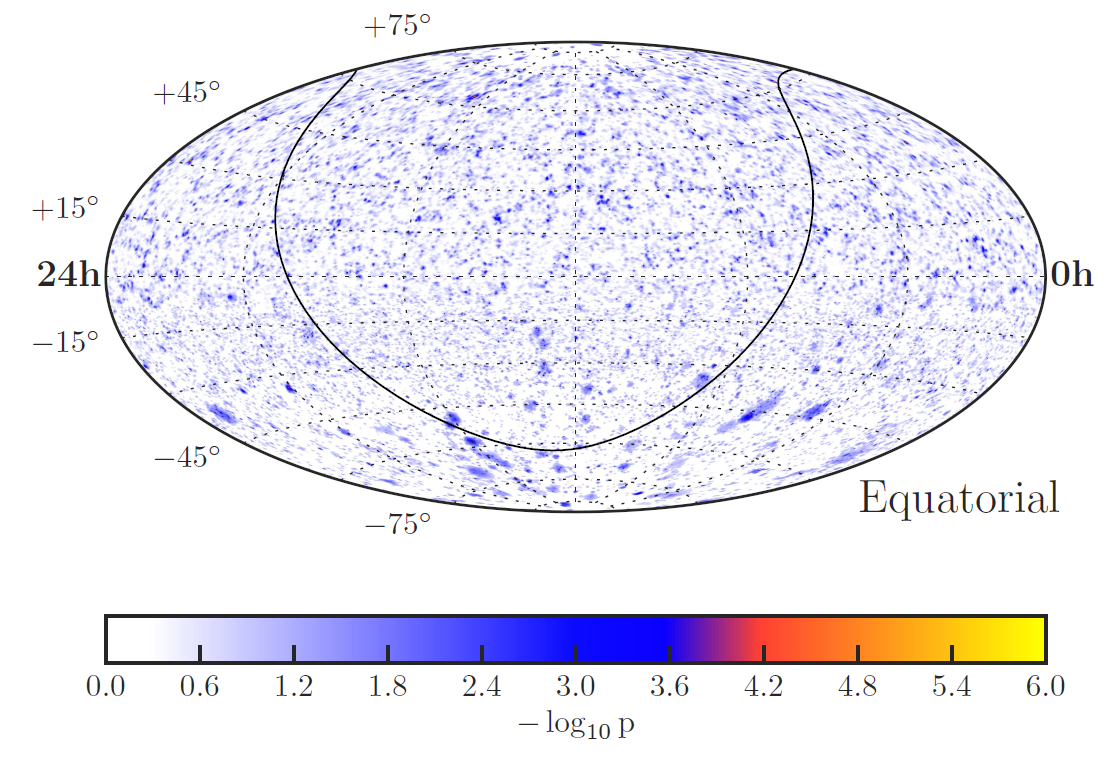
\includegraphics[keepaspectratio,height=14cm]{icecube-skymap-7years}
\end{center}

\Transcb{yellow}{blue}{Neutrinos van kosmische gammaflitsen}
\twocolumn

\vspace*{1cm}

\begin{itemize}
\item Signalen zijn atm. achtergrond $\nu$
\item[] Niet te onderscheiden van kosm. $\nu$\\[3mm]
\item[] \colorbox{yellow}{Kijk naar kortstondige explosies}\\
\item[] Specifieke plaats en tijd (satelliet)
\item[] $\rightarrow$ nagenoeg geen achtergrond
\item[$\ast$] {\blue IIHE movie}
\end{itemize}

\newpage

\begin{center}
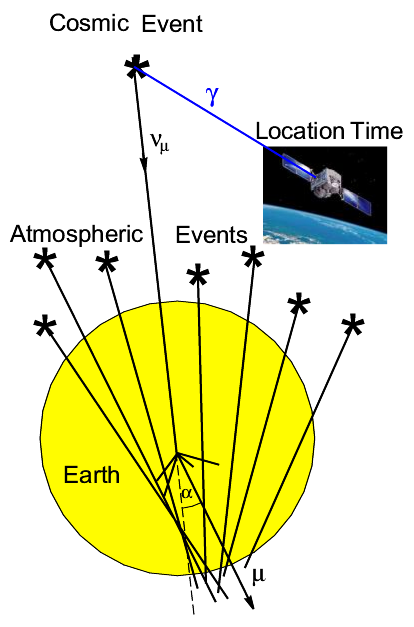
\includegraphics[keepaspectratio,height=16cm]{atm-bkg}
\end{center}

\Transcb{yellow}{blue}{The Muppets on Ice}
\twocolumn
\begin{center}
{\blue Tue 09-aug-2011 07:23:18 UTC}\\
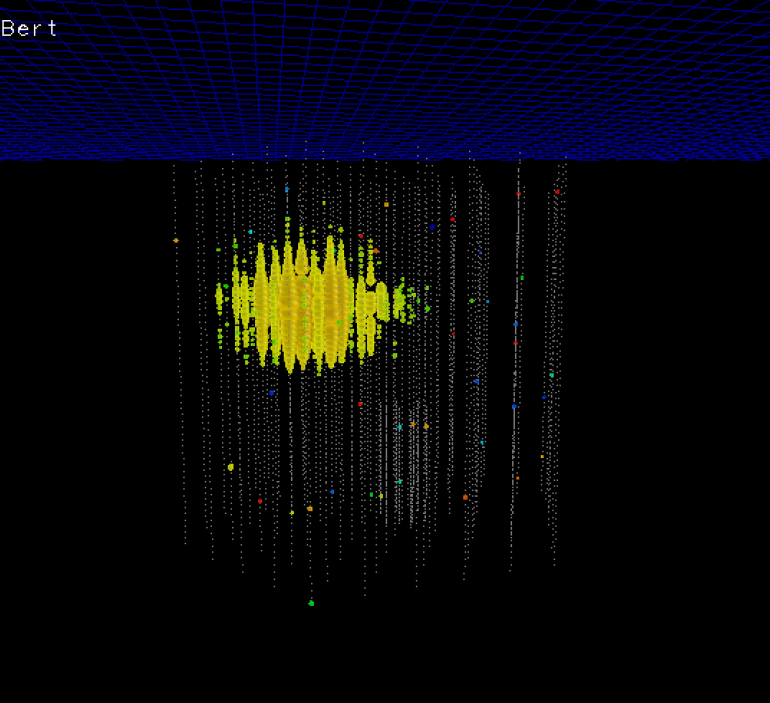
\includegraphics[keepaspectratio,width=13cm]{bert}\\
$1.04 \pm 0.16$ PeV
\end{center}
{\blue Atmosferische $\nu$ achtergrond ?}

\newpage

\begin{center}
{\blue Tue 03-jan-2012 03:34:01 UTC}\\
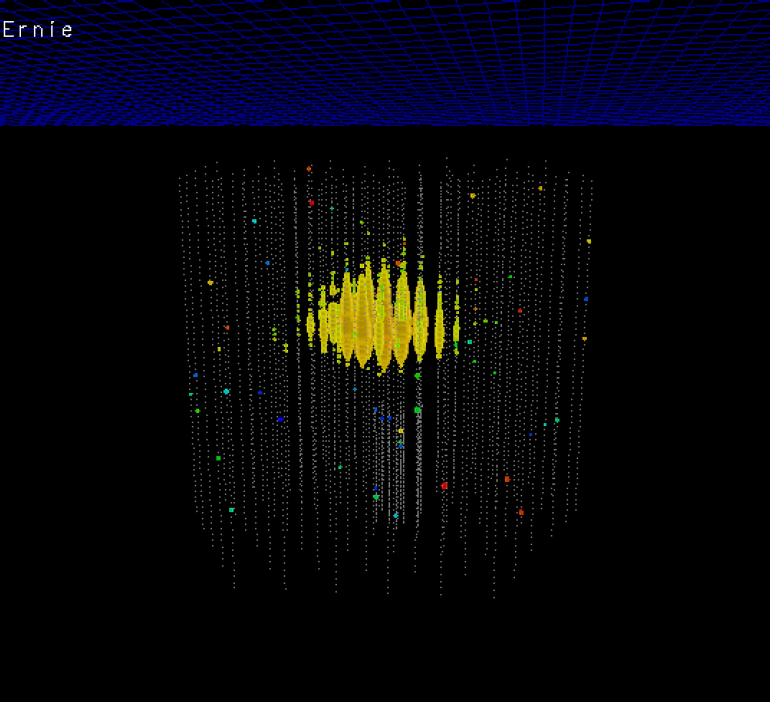
\includegraphics[keepaspectratio,width=13cm]{ernie}\\
$1.14 \pm 0.17$ PeV
\end{center}
{\blue Slechts ca. 0.3\% kans op achtergrond}

\Tr
\twocolumn[\begin{center}{\blue Nog 52 additionele events gevonden}\end{center}]
%
\begin{center}
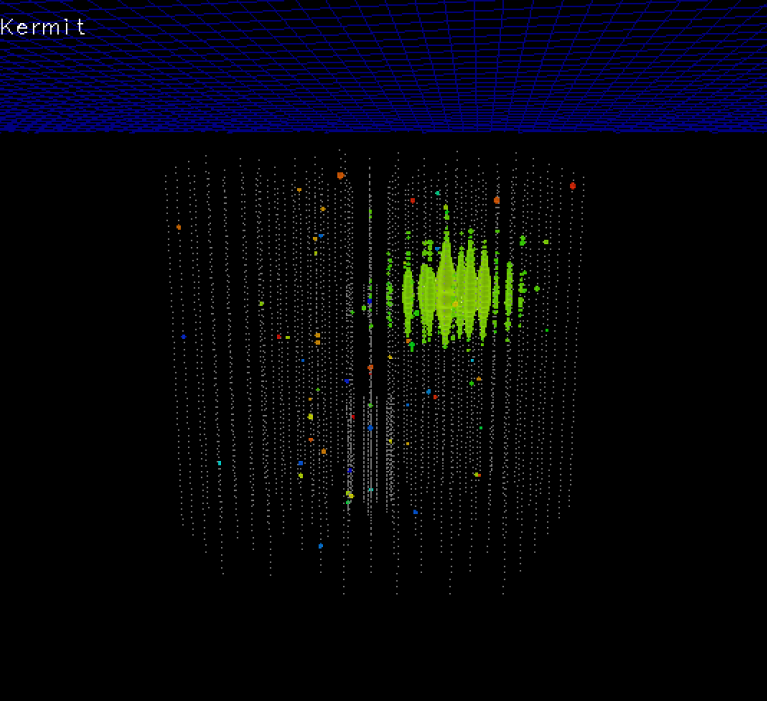
\includegraphics[keepaspectratio,width=13cm]{kermit}
\end{center}

\newpage

\begin{center}
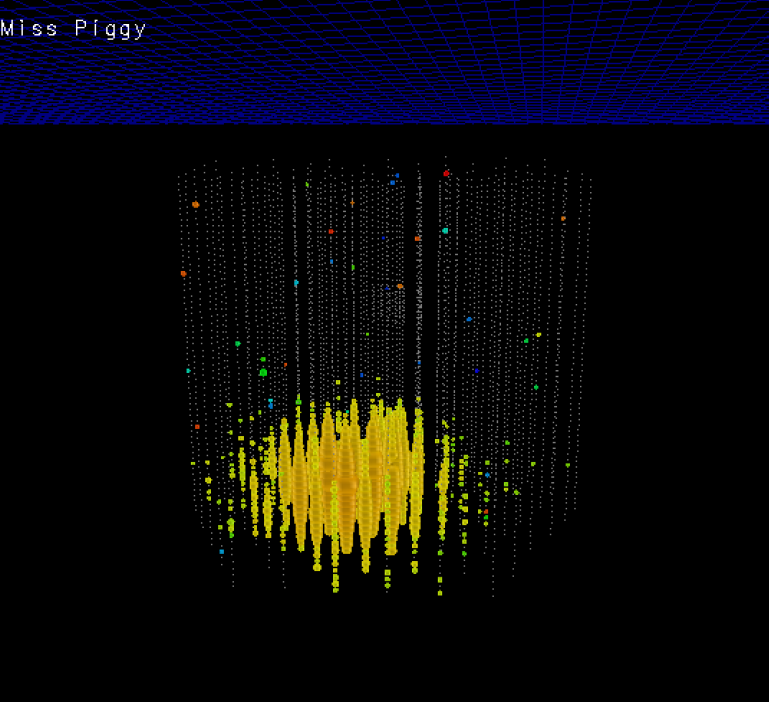
\includegraphics[keepaspectratio,width=13cm]{miss-piggy}
\end{center}

\Tr
\twocolumn[\begin{center}{\blue Ook enkele $\mu$ spoor signaturen}\end{center}]
%
\begin{center}
\includegraphics[keepaspectratio,width=13cm]{dr-strangepork}
\end{center}

\newpage

\begin{center}
\includegraphics[keepaspectratio,width=13cm]{gonzo-the-great}
\end{center}

\Tr
\twocolumn[\begin{center}{\blue Onze huidige kampioen}\end{center}]
%
\begin{center}
\includegraphics[keepaspectratio,width=13cm]{big-bird}\\
$2.00 \pm 0.25$ PeV
\end{center}

\newpage

\begin{center}
\includegraphics[keepaspectratio,height=12cm]{big-bird-photo}\\
Big Bird
\end{center}

\Tr
\onecolumn
\begin{center}
{\blue Energie distributie van de 54 events}
\end{center}
\includegraphics[keepaspectratio,width=13.5cm]{hese-e}
\includegraphics[keepaspectratio,width=13.5cm]{hese-decl-vs-e}
\begin{center}
\colorbox{yellow}{Aanduiding voor kosmische hoog-energetische neutrino's}
\end{center}

\Tr
\onecolumn
\begin{center}
{\blue Herkomst van de 54 events}\\[5mm]
\includegraphics[keepaspectratio,width=20cm]{hese-skymap-gal}\\
\colorbox{yellow}{Geen bewijs voor puntbron(nen)}
\end{center}

\Transcb{yellow}{blue}{Vooruitzichten}
\onecolumn
\begin{itemize}
\item \colorbox{yellow}{IceCube : 's Werelds grootste neutrino observatorium op de Zuidpool}
\item[] De volledige IceCube detector is sinds december 2010 in bedrijf
\item[] IceCube sensoren werken naar behoren (Maanschaduw, hemelkaart)
\item \colorbox{yellow}{Zeer gedetailleerd onderzoek van de "neutrino hemel"}
\item[] Valt in tijd mooi samen met satelliet waarnemingen (Swift, Fermi)
\item[] $\rightarrow$ Perfect voor GRB onderzoek
\item \colorbox{yellow}{Wereldprimeur : Kosmische hoog-energetische neutrino's ontdekt}
\item[] \begin{center}{\blue De geboorte van Neutrino Astronomie}\end{center}
\item {\red Onderzoek aan de VUB :}
\item[] Nieuwe methode voor detectie van GRB neutrino's
\item[] Onderzoek naar neutrino productie in zonnevlammen
\item[] Nieuw idee voor neutrino detectie van actieve melkwegkernen 
\end{itemize}
%
\begin{center}
\colorbox{yellow}{Er breken zeer interessante tijden aan voor onze Astrodeeltjes Fysica !}
\end{center}


\end{document}